%====================================================
% UNIVERSITY OF ECONOMICS HO CHI MINH CITY (UEH)
% GRADUATE ACADEMIC TEMPLATE
% LANGUAGE: VIETNAMESE
% COMPILE: XeLaTeX + Biber
%====================================================

\documentclass[12pt,a4paper]{report}

%----------------------------------------------------
% COLOR THEME (UEH)
%----------------------------------------------------
\usepackage{xcolor}
\definecolor{uehblue}{RGB}{0,70,127}
\definecolor{uehgray}{RGB}{80,80,80}

%----------------------------------------------------
% LANGUAGE & FONT
%----------------------------------------------------
\usepackage{fontspec} 
\setmainfont[Ligatures=TeX]{Times New Roman} 

\usepackage{polyglossia}
\setmainlanguage{vietnamese}
\setotherlanguage{english}

%----------------------------------------------------
% PAGE LAYOUT
%----------------------------------------------------
\usepackage{geometry}
\geometry{
	left=3cm,
	right=2.5cm,
	top=3cm,
	bottom=3cm
}

\usepackage{setspace}
\onehalfspacing

\setlength{\parindent}{0pt}
\setlength{\parskip}{6pt}

%----------------------------------------------------
% CORE PACKAGES
%----------------------------------------------------
\usepackage{graphicx}
\graphicspath{{figures/}}

\usepackage{booktabs}
\usepackage{longtable}
\usepackage{amsmath,amssymb}
\usepackage{float}

\usepackage{subcaption}
\usepackage{tabularx}
\usepackage{multirow}  

%\usepackage{csquotes}

%----------------------------------------------------
% FIGURE & TABLE CAPTION
%----------------------------------------------------
\usepackage{caption}
\captionsetup{
	font=small,
	labelfont=bf,
	justification=raggedright,
	singlelinecheck=false
}

%----------------------------------------------------
% HYPERLINKS
%----------------------------------------------------
\usepackage{hyperref}
\hypersetup{
	colorlinks=true,
	linkcolor=black,
	citecolor=uehblue,
	urlcolor=blue
}

%----------------------------------------------------
% HEADER & FOOTER – UEH
%----------------------------------------------------
\usepackage{fancyhdr}
\usepackage{lastpage}

\pagestyle{fancy}
\fancyhf{}

% Header
\fancyhead[L]{\small\textit{Đại học Kinh tế Thành phố Hồ Chí Minh}}

\fancyhead[R]{\small\textit{Niên khóa 2025--2026}}

% Footer
\fancyfoot[L]{
\includegraphics[height=0.8cm]{logoueh.png}}
\fancyfoot[C]{\small\textit{Các chủ đề nghiên cứu trong kinh tế học}}
\fancyfoot[R]{\small Trang \thepage\ | \pageref{LastPage}}

\renewcommand{\headrulewidth}{0.4pt}
\renewcommand{\footrulewidth}{0pt}

%----------------------------------------------------
% SECTION FORMAT
%----------------------------------------------------
\usepackage{titlesec}
\titleformat{\section}{\bfseries\large}{\thesection.}{0.5em}{}
\titleformat{\subsection}{\bfseries}{\thesubsection}{0.5em}{}
\titleformat{\subsubsection}{\itshape}{\thesubsubsection}{0.5em}{}

%----------------------------------------------------
% BIBLIOGRAPHY – APA / HARVARD
%----------------------------------------------------
\usepackage[
backend=biber,
style=authoryear,
sorting=nyt,
maxcitenames=2,
maxbibnames=99,
doi=true,
url=true,
isbn=false
]{biblatex}

\addbibresource{references.bib}

%====================================================
% DOCUMENT START
%====================================================
\begin{document}
	
%====================================================
	% TITLE PAGE – UEH STANDARD FORMAT
%====================================================
	\begin{titlepage}
		\centering
		\vspace*{0.5cm}
		
		{\large \textbf{BỘ GIÁO DỤC VÀ ĐÀO TẠO}}\\
		{\Large \textbf{\textcolor{blue}{ĐẠI HỌC KINH TẾ THÀNH PHỐ HỒ CHÍ MINH}}}\\
		\vspace{0.2cm}
		\textbf{TRƯỜNG KINH TẾ, LUẬT VÀ QUẢN LÝ NHÀ NƯỚC}\\
		\vspace{1.5cm}
		
		% Anh nhớ để file ảnh logoueh.png cùng thư mục với file TeX nhé
		
\includegraphics[width=4.5cm]{logoueh.png}\\[2cm] 
		
		{\large \textbf{BÀI NGHIÊN CỨU KẾT THÚC HỌC PHẦN}}\\[0.5cm]
		{\large \textbf{Môn học: CÁC CHỦ ĐỀ NGHIÊN CỨU TRONG KINH TẾ HỌC}}\\[1.5cm]
		
		% Khung tên đề tài
		\begin{minipage}{0.9\textwidth}
			\centering
			\textbf{\LARGE TÁC ĐỘNG CỦA TIẾP CẬN TÍN DỤNG ĐẾN GÁNH NẶNG NHÀ Ở CỦA HỘ GIA ĐÌNH ĐÔ THỊ VIỆT NAM}\\[0.6cm]
			\textit{\Large Bằng chứng thực nghiệm từ mô hình tác động xử lý nội sinh}
		\end{minipage}
		
		\vspace{2.5cm}
		
		\begin{flushleft}
	\textbf{Học viên:} Trương Nhật Duy\\
	\textbf{Mã học viên:} [ID redacted]\\
	\textbf{Chuyên ngành:} Kinh tế Phát triển\\
	
\end{flushleft}
	
		{\large \textbf{TP. Hồ Chí Minh, Năm 2026}}
	\end{titlepage}
	
%====================================================
	% TABLE OF CONTENTS
%====================================================
	\tableofcontents
	\newpage	
%====================================================
% MAIN CONTENT
	%====================================================
	%====================================================
	%=============================
% DANH MỤC BẢNG
	%=============================
	\listoftables
	\addcontentsline{toc}{chapter}{Danh mục bảng}
	%=============================
	% DANH MỤC HÌNH
	%=============================
	\listoffigures
	\addcontentsline{toc}{chapter}{Danh mục hình}
	%=============================
	% ABSTRACT
	%====================================================
	\chapter*{Tóm tắt}
	\addcontentsline{toc}{chapter}{Tóm tắt}
	
	Nghiên cứu này phân tích các rào cản trong việc tiếp cận tín dụng và đánh giá tác động thực sự của khả năng tiếp cận tín dụng đến gánh nặng chi phí nhà ở của nhóm hộ gia đình có thu nhập trung bình thấp (Missing Middle). Dựa trên bộ dữ liệu điều tra VHLSS năm 2024 gồm 10.246 quan sát, nghiên cứu áp dụng mô hình Hiệu ứng xử lý nội sinh (Etregress) kết hợp với các biến công cụ (IV) như hiệu ứng đồng trang lứa và mạng lưới xã hội. Phương pháp này giúp khắc phục triệt để hiện tượng sai lệch chọn mẫu và tính nội sinh, đồng thời bảo toàn tối đa cỡ mẫu so với các mô hình truyền thống.
	
	Kết quả thực nghiệm cho thấy việc tiếp cận tín dụng hiện tại không làm giảm gánh nặng nhà ở của nhóm Missing Middle một cách có ý nghĩa thống kê. Thêm vào đó, việc cố gắng sở hữu tài sản (nhà ở hoặc tài sản thế chấp) thực chất lại làm tăng gánh nặng tài chính do các chi phí duy trì đi kèm. Điều này phản ánh thực tế rằng các khoản tín dụng hiện hành chủ yếu chỉ giải quyết nhu cầu thanh khoản ngắn hạn, thay vì tạo ra đòn bẩy tài chính làm thay đổi vị thế chi trả dài hạn.
	
	Ngược lại, năng lực tạo thu nhập và hiệu ứng kinh tế nhờ quy mô hộ gia đình mới là những yếu tố cốt lõi giúp giảm tải áp lực chi phí nhà ở một cách mạnh mẽ nhất. Nút thắt của bài toán nhà ở đối với nhóm Missing Middle nằm ở khả năng sinh lời của sức lao động hơn là sự thiếu hụt các khoản nợ vay.
	
	Từ các bằng chứng định lượng, nghiên cứu này đề xuất một sự chuyển dịch trong trọng tâm chính sách đối với nhóm thu nhập trung bình thấp tại đô thị. Thay vì thuần túy phụ thuộc vào việc nới lỏng tín dụng mua nhà, Nhà nước cần ưu tiên phát triển các mô hình nhà ở xã hội cho thuê nhằm giảm trực tiếp tử số chi phí, đồng thời thúc đẩy các chính sách hỗ trợ việc làm và sinh kế để gia tăng thu nhập cốt lõi cho hộ gia đình.
	
			
	% ================= CHƯƠNG 1 =================
	\chapter{Giới thiệu}
	
	\section{Tính cấp thiết của đề tài}
	
	Quá trình đô thị hóa nhanh chóng tại Việt Nam trong hai thập niên gần đây đã tạo ra động lực tăng trưởng kinh tế mạnh mẽ, đồng thời đặt ra những thách thức lớn về an sinh xã hội, đặc biệt là vấn đề tiếp cận nhà ở phù hợp cho nhóm dân cư thu nhập thấp và trung bình tại các đô thị lớn. Theo Tổng cục Thống kê, tỷ lệ dân số đô thị của Việt Nam đã tăng từ dưới 25\% năm 2000 lên trên 40\% vào năm 2023, kéo theo áp lực ngày càng gia tăng lên thị trường nhà ở và hạ tầng đô thị \parencite{VietnamGSO2023}.
	
	Mặc dù Chính phủ Việt Nam đã ban hành nhiều chính sách nhằm thúc đẩy phát triển nhà ở xã hội và mở rộng tín dụng ưu đãi cho người thu nhập thấp, tiêu biểu là gói tín dụng 120.000 tỷ VND theo Nghị quyết 33/NQ-CP \textcite{NQ33CP2022}, khả năng tiếp cận tín dụng nhà ở chính thức của các hộ gia đình đô thị thu nhập thấp vẫn ở mức rất hạn chế. Bằng chứng thực tế cho thấy khoảng cách đáng kể giữa mục tiêu chính sách và kết quả triển khai. Tỷ lệ giải ngân của gói tín dụng này chỉ đạt 2,37\% (tương đương 2.845 tỷ VND) tính đến tháng 3/2025 sau gần ba năm thực hiện, và tăng lên 4,3\% (5.160 tỷ VND) vào tháng 11/2025 \parencite{CafeLand2025,CafeF2025}. Mức giải ngân này thấp hơn khoảng mười lần so với benchmark triển khai tín dụng nhà ở ưu đãi giai đoạn 2016–2020 của Agribank (38\%), cho thấy sự tồn tại của các rào cản mang tính cấu trúc trong thị trường tín dụng nhà ở \parencite{SBV2025}. 
	
	Từ góc độ kinh tế học phát triển, sự ách tắc này thường được lý giải thông qua lý thuyết về bất cân xứng thông tin \parencite{Stiglitz1981}. Các tổ chức tín dụng có xu hướng hạn chế cho vay đối với nhóm khách hàng có thu nhập phi chính thức hoặc thiếu tài sản đảm bảo. Điều này tạo ra rào cản lớn đối với nhóm hộ gia đình Missing Middle, những hộ có thu nhập vượt ngưỡng hỗ trợ an sinh xã hội khẩn cấp nhưng lại không đủ điều kiện tiếp cận tín dụng thương mại chính thức.
	
	Tuy nhiên, một câu hỏi lớn hơn và ít được kiểm chứng tại Việt Nam là: Liệu việc tiếp cận được tín dụng và sở hữu tài sản có thực sự giúp nhóm lao động yếu thế giảm bớt gánh nặng chi phí nhà ở, hay chỉ đơn thuần chuyển từ áp lực này sang một gánh nặng nợ nần khác? Trong bối cảnh giá bất động sản đô thị leo thang, việc cố gắng sở hữu nhà thông qua đòn bẩy tài chính có thể khiến các hộ gia đình rơi vào bẫy thanh khoản, làm suy giảm trầm trọng khả năng chi tiêu cho y tế, giáo dục và phúc lợi tổng thể.
	
	Do đó, việc nghiên cứu một cách hệ thống không chỉ về rào cản tiếp cận tín dụng, mà quan trọng hơn là đánh giá tác động thực sự của tín dụng (khi đã kiểm soát các yếu tố nội sinh) đến gánh nặng nhà ở của hộ gia đình thu nhập thấp đô thị là vô cùng cấp thiết. Nghiên cứu này nhằm lấp đầy khoảng trống đó bằng cách kết hợp phân tích định lượng vi mô với khung lý thuyết kinh tế tài chính, từ đó định hình lại tư duy chính sách: từ việc thuần túy cho vay thông qua các gói tín dụng sang các giải pháp bền vững hơn về cấu trúc thu nhập và nguồn cung nhà ở.
	
	\section{Câu hỏi nghiên cứu}
	
	Dựa trên bối cảnh và mục tiêu nghiên cứu đã nêu, nghiên cứu tập trung trả lời hai câu hỏi cốt lõi sau:
	
	\begin{enumerate}
		\item Những yếu tố nào quyết định khả năng tiếp cận tín dụng của hộ gia đình đô thị tại Việt Nam?
		
		\item Việc tiếp cận tín dụng và sở hữu tài sản bảo đảm có thực sự làm giảm gánh nặng chi phí nhà ở của nhóm Missing Middle hay không?
	\end{enumerate}
	
	\section{Đối tượng và phạm vi nghiên cứu}
	
	Đối tượng nghiên cứu của bài viết là các hộ gia đình sinh sống tại khu vực đô thị ở Việt Nam. Nghiên cứu tập trung vào các hộ gia đình thuộc nhóm ngũ phân vị thu nhập thứ nhất, thứ hai và thứ ba, đại diện cho nhóm lao động có thu nhập thấp và trung bình thấp (Missing Middle), nhóm chịu sự tác động lớn nhất giữa nhu cầu an cư và giới hạn tài chính.
	
	Về phạm vi dữ liệu, nghiên cứu sử dụng bộ dữ liệu Khảo sát Mức sống Dân cư Việt Nam (Vietnam Household Living Standards Survey -- VHLSS) năm 2024 \parencite{VHLSS2024} do Tổng cục Thống kê thực hiện. Đây là bộ dữ liệu vi mô có tính đại diện quốc gia, cung cấp thông tin chi tiết về thu nhập, chi tiêu, điều kiện nhà ở, và khả năng tiếp cận các dịch vụ tài chính của hộ gia đình.
	
	Về phạm vi không gian và thời gian, nghiên cứu giới hạn trong khu vực đô thị và sử dụng dữ liệu cắt ngang tại thời điểm năm 2024. Phạm vi này cho phép phản ánh chính xác nhất cấu trúc hiện tại của thị trường tín dụng và áp lực chi phí sinh hoạt tại các trung tâm kinh tế của Việt Nam.

% ================= CHƯƠNG 2 =================
\chapter{Cơ sở lý thuyết và Tổng quan nghiên cứu}

\section{Thị trường tín dụng và Tiêu dùng hộ gia đình}

\subsection{Thông tin bất cân xứng và Hạn chế tín dụng}

Trong kinh tế học tài chính, hạn chế tín dụng là một hiện tượng cấu trúc phổ biến khi thị trường vốn vận hành dưới điều kiện thông tin không hoàn hảo. Nghiên cứu của \textcite{Stiglitz1981} chỉ ra rằng, khi tồn tại bất cân xứng thông tin, các ngân hàng thương mại không thể sử dụng lãi suất như một công cụ duy nhất để rào cản rủi ro. Việc tăng lãi suất quá mức sẽ dẫn đến vấn đề lựa chọn đối nghịch. Thay vào đó, ngân hàng ưu tiên cấp vốn dựa trên tài sản đảm bảo và phân phối hạn mức tín dụng. Hệ quả là một bộ phận lớn khách hàng, đặc biệt là nhóm thu nhập trung bình thấp ở đô thị (nhóm Missing Middle), bị loại khỏi hệ thống tín dụng chính thức dù họ sẵn sàng trả mức lãi suất cao hơn.


\subsection{Giả thuyết vòng đời và Nghịch lý nợ tiêu dùng}

Để lý giải hành vi vay mượn của hộ gia đình, Giả thuyết vòng đời (Life-Cycle Hypothesis) của \textcite{Modigliani1963} cho rằng con người có xu hướng vay mượn khi còn trẻ để làm mượt tiêu dùng (consumption smoothing) và tích lũy tài sản (mua nhà), sau đó trả nợ vào giai đoạn đỉnh cao thu nhập. 

\begin{figure}[htbp]
	\centering
	\includegraphics[width=0.75\textwidth]{lifecycle_hypothesis.png}
	\caption{Mô hình Giả thuyết vòng đời và hành vi làm mượt tiêu dùng}
	\label{fig:lifecycle}
	\subcaption*{\footnotesize \textit{Nguồn: \textcite{Modigliani1963}.}}
\end{figure}

Tuy nhiên, khi phân tích sâu vào bản chất tín dụng, cần phân định rạch ròi giữa tín dụng sản xuất (Productive credit) và tín dụng tiêu dùng/nhà ở (Consumptive credit). Nếu tín dụng sản xuất giúp tạo ra dòng tiền mới để bù đắp chi phí vốn, thì tín dụng nhà ở lại đòi hỏi dòng tiền sẵn có từ thu nhập cốt lõi để duy trì. Do đó, việc mở rộng tín dụng nhà ở cho nhóm thu nhập thấp, nếu không đi kèm với sự gia tăng năng suất lao động, sẽ dẫn đến Nghịch lý nợ tiêu dùng. Tại đây, tín dụng không làm giảm gánh nặng tài chính mà thực chất chỉ là hành vi chuyển hóa rủi ro thanh khoản ngắn hạn thành việc mất thanh khoản và rủi ro vỡ nợ dài hạn.


\section{Đòn bẩy tài chính và bẫy tài sản}

Khung lý thuyết về tài sản và tín dụng tại các nước đang phát triển từng chịu ảnh hưởng sâu sắc bởi quan điểm lạc quan của Hernando de Soto \parencite{deSoto2000}. Ông lập luận rằng việc hợp pháp hóa tài sản nhà đất để làm thế chấp sẽ giúp người nghèo giải phóng nguồn vốn trói buộc và thoát nghèo. Mặc dù vậy, sự phát triển của kinh tế học hành vi và kinh tế phát triển hiện đại đã thách thức mạnh mẽ góc nhìn này.

Thông qua các Thử nghiệm ngẫu nhiên có đối chứng (RCTs) quy mô lớn, \textcite{Banerjee2015} và \textcite{Karlan2010} chứng minh rằng việc mở rộng quyền tiếp cận tín dụng không tự động tạo ra sự gia tăng đáng kể về thu nhập hay tiêu dùng dài hạn. Tín dụng chủ yếu chỉ giúp hộ gia đình chống chịu với các cú sốc thanh khoản tạm thời.

Đặc biệt, trong tài chính nhà ở, \textcite{Mian2014} với tác phẩm nền tảng \textit{House of Debt} đã chỉ ra rằng đòn bẩy tài chính của hộ gia đình quá mức chính là nguyên nhân cốt lõi dẫn đến sự suy yếu tài chính. Khi hộ gia đình cố gắng vay mượn để sở hữu tài sản trong bối cảnh khủng hoảng khả năng chi trả đô thị \textcite{Glaeser2018}, họ rất dễ rơi vào bẫy tài sản. Bẫy tài sản hình thành khi việc sở hữu nhà đi kèm với các chi phí chìm khổng lồ: Thuế, phí bảo trì, nghĩa vụ trả nợ gốc lãi và chi phí cơ hội của dòng tiền. Khi các chi phí này vượt quá thặng dư thu nhập, ngôi nhà thay vì là bệ phóng tài chính lại biến thành một gánh nặng. Hơn nữa, theo \textit{Giả thuyết Oswald} \parencite{Oswald1996}, việc gắn chặt vào một tài sản cố định làm giảm tính linh hoạt của lao động, gia tăng rủi ro thất nghiệp và làm suy giảm nghiêm trọng chất lượng cuộc sống thực tế.

\section{Tổng quan các nghiên cứu thực nghiệm}

Các bằng chứng thực nghiệm gần đây đã củng cố mạnh mẽ cho sự tồn tại của Nghịch lý nợ tiêu dùng và Bẫy tài sản. Tại các thị trường phát triển, nghiên cứu của \textcite{Carozzi2024} về chương trình Help to Buy chỉ ra rằng các chính sách nới lỏng tín dụng thực chất chỉ làm thổi phồng giá nhà thay vì tăng nguồn cung, khiến khả năng chi trả ngày càng tồi tệ hơn \parencite{LarsonMartinez2025, Brown2015}. Thậm chí, \textcite{WillRenz2023} phát hiện ra rằng việc mang nợ thế chấp (Mortgage) tác động tiêu cực đến sự hài lòng về cuộc sống của hộ gia đình tại Đức, bất chấp việc họ đã đạt được mục tiêu sở hữu nhà.

Bổ sung thêm góc nhìn từ các cuộc khủng hoảng, nghiên cứu mang tính bước ngoặt của \textcite{MianSufi2009} cảnh báo hệ lụy nghiêm trọng của việc nới lỏng tín dụng thiếu kiểm soát. Bằng dữ liệu không gian, các tác giả phát hiện dòng tín dụng thế chấp tại Mỹ từng tăng đột biến ở các khu vực "dưới chuẩn" bất chấp thu nhập thực tế tại đây đang suy giảm. Cú sốc cung tín dụng (\textit{credit supply shock}) này đã thổi bùng bong bóng giá nhà và dẫn đến làn sóng vỡ nợ diện rộng. Bằng chứng này củng cố một lập luận cốt lõi: khi nguồn cung tín dụng bị ngắt kết nối với năng lực trả nợ, đòn bẩy tài chính sẽ trở thành rủi ro thay vì bệ phóng an sinh. 

Tại bối cảnh các nước đang phát triển, bằng chứng từ Mỹ Latinh và Châu Phi \parencite{Arrieta2005} và \parencite{Edwin2023} chứng minh rằng việc sử dụng tài sản nhà đất làm thế chấp giúp người thu nhập thấp vượt qua rào cản tín dụng, nhưng lại làm tăng vọt gánh nặng tài chính hàng tháng. Tương tự tại Châu Á, \textcite{Sato2024} và \textcite{Syed2025} nhấn mạnh rằng tín dụng nhà ở cho nhóm yếu thế chỉ cải thiện cảm nhận về an sinh chứ không làm giảm áp lực chi trả thực tế; thu nhập cốt lõi mới là yếu tố quyết định.

Riêng tại Việt Nam, nghiên cứu của \textcite{Nguyen2016} chỉ ra rằng tiếp cận tín dụng không phải lúc nào cũng làm tăng mức độ hài lòng của hộ gia đình mua nhà ở xã hội do áp lực duy trì chi phí. Nghiên cứu thực nghiệm tại TP. Hà Nội của \textcite{BuiTruong2023} và báo cáo SBV \textcite{SBV2025} đã nỗ lực đánh giá rào cản tín dụng, nhưng thường chưa xử lý triệt để tính nội sinh của quyết định đi vay đối với gánh nặng chi phí, dẫn đến các kết luận có phần lạc quan về vai trò của tín dụng. \textcite{WorldBank2024} sử dụng VHLSS 2018-2022 xác nhận chính xác hiện tượng: Tiếp cận tín dụng nhà ở xã hội gặp rào cản cấu trúc nghiêm trọng, thường chỉ cải thiện khả năng mua nhà chứ không giảm gánh nặng tài chính dài hạn cho nhóm Missing Middle. Trên thực tế, tỷ lệ giải ngân thấp (dưới 5\%) của gói tín dụng 120.000 tỷ VND phản ánh không chỉ rào cản từ phía cung, mà còn là sự e ngại rủi ro nợ nần, rơi vào bẫy tài sản từ chính phía cầu. 

Tổng quan các tài liệu nghiên cứu trên không chỉ cung cấp cơ sở để lý giải sự ách tắc của các gói tín dụng ưu đãi tại Việt Nam (khi người dân e ngại vay mượn do thu nhập không tăng kịp giá nhà), mà còn khẳng định sự cần thiết của việc áp dụng mô hình vi mô như \textit{etregress} trong nghiên cứu này để bóc tách chính xác quyết định tự chọn tham gia thị trường nợ của từng hộ gia đình đặc biệt trong bối cảnh lãi suất cho vay tăng cao và siết tín dụng, và cho vay bất động sản tại thời điểm bài nghiên cứu này tiến hành.

\subsection{Khoảng trống nghiên cứu}
Từ lược khảo lý thuyết và thực nghiệm, nghiên cứu nhận diện ba khoảng trống chính:
\begin{itemize}
	\item \textbf{Về mặt thực nghiệm:} Thiếu các nghiên cứu định lượng kiểm định trực tiếp tác động thực sự của tín dụng đến tỷ lệ gánh nặng chi phí nhà ở/thu nhập tại Việt Nam, thay vì chỉ dừng lại ở việc phân tích rào cản tiếp cận.
	\item \textbf{Về mặt phương pháp:} Các nghiên cứu trước đây chủ yếu sử dụng OLS hoặc mô hình Heckman. Tuy nhiên, Heckman bộc lộ điểm yếu làm mất dữ liệu khi biến kết quả được quan sát trên toàn bộ tổng thể. Việc áp dụng mô hình Hiệu ứng xử lý nội sinh (Endogenous Treatment Effects) để kiểm soát sai lệch chọn mẫu là một khoảng trống lớn về phương pháp luận.
	\item \textbf{Về cơ chế truyền dẫn:} Sự thiếu vắng vai trò của các biến số phi chính thức như mạng lưới xã hội (Social network) và hiệu ứng đồng trang lứa (Peer effect) trong việc định hình quyết định vay mượn của hộ gia đình đô thị.
\end{itemize}

Nhằm lấp đầy các khoảng trống này, nghiên cứu sử dụng dữ liệu vi mô quy mô lớn (VHLSS 2024), áp dụng mô hình Etregress, và sử dụng các yếu tố xã hội làm biến công cụ để đo lường chính xác tác động nhân quả của tín dụng.


\section{Khung phân tích nghiên cứu và mô hình}

Để bóc tách tính nội sinh của quyết định vay vốn, nghiên cứu áp dụng mô hình Etregress được ước lượng bằng phương pháp Full Information Maximum Likelihood. Khác với quy trình Heckman hai bước tự động loại bỏ các quan sát không can thiệp ở phương trình kết quả, mô hình Etregress cho phép giữ nguyên 100\% cỡ mẫu, qua đó cung cấp các ước lượng hiệu quả và vững chắc hơn.

Hệ phương trình toán học bao gồm:

1. \textbf{Phương trình kết quả (Outcome Equation - Gánh nặng nhà ở):}
\begin{equation}
	Burden_i = \beta_0 + \beta_1 CreditAccess_i + \beta_2 \ln(Income_i) + \beta_3 HHSize_i + \beta_4 Collateral_i + \varepsilon_i 
\end{equation}

2. \textbf{Phương trình xử lý nội sinh (Treatment Equation - Xác suất vay vốn):}
\begin{equation}
	CreditAccess_i^* = \gamma_0 + \gamma_1 \ln(Income_i) + \gamma_2 Informal_i + \gamma_3 Collateral_i + \gamma_4 Z_i + u_i 
\end{equation}

Trong đó, biến quan sát $CreditAccess_i = 1$ (hộ gia đình có đi vay) nếu biến tiềm ẩn $CreditAccess_i^* > 0$, và bằng $0$ nếu ngược lại. 

Điểm mấu chốt cấu thành chiến lược nhận dạng (identification strategy) của mô hình là vector biến công cụ $Z_i$ (bao gồm \textit{peer\_effect} và \textit{social\_network}) được đưa riêng vào phương trình xử lý. Các biến này thỏa mãn điều kiện ngoại sinh nghiêm ngặt: chúng làm giảm chi phí tìm kiếm thông tin, qua đó tác động mạnh mẽ đến quyết định đi vay (Relevance condition), nhưng không tác động trực tiếp đến gánh nặng chi phí nhà ở sau khi đã kiểm soát mức thu nhập và quy mô hộ gia đình (Exclusion restriction).

Về mặt thống kê, sai số $\varepsilon_i$ và $u_i$ được giả định tuân theo phân phối chuẩn nhị chiều (Bivariate Normal Distribution) với hiệp phương sai $\rho$. Nếu quyết định đi vay bị ảnh hưởng bởi các yếu tố ẩn không quan sát được (ví dụ: mức độ ưa thích rủi ro của chủ hộ), $\rho$ sẽ khác $0$, khiến ước lượng OLS thông thường bị chệch. Cấu trúc mô hình \textit{etregress} sẽ đo lường và hiệu chỉnh triệt để phần dư nội sinh này.
		

% ================= CHƯƠNG 3 =================
\chapter{Phương pháp nghiên cứu và Dữ liệu}

\section{Dữ liệu nghiên cứu}

Nghiên cứu sử dụng bộ dữ liệu VHLSS năm 2024 do Tổng cục Thống kê Việt Nam (GSO) thực hiện và công bố. Đây là bộ dữ liệu vi mô đại diện cấp quốc gia, cung cấp thông tin toàn diện về đặc điểm nhân khẩu học, thu nhập, chi tiêu, điều kiện nhà ở và khả năng tiếp cận tín dụng của các hộ gia đình.

Để tập trung giải quyết câu hỏi nghiên cứu, mẫu dữ liệu được giới hạn ở các hộ gia đình sinh sống tại khu vực đô thị và thuộc các ngũ phân vị thu nhập từ 1 đến 3. Đây là nhóm đại diện cho tầng lớp thu nhập thấp và trung bình thấp (nhóm Missing Middle), những người có thu nhập vượt ngưỡng nghèo chuẩn nhưng lại không đủ tiềm lực tài chính để tiếp cận nhà ở thương mại. 

Sau quá trình làm sạch dữ liệu và loại bỏ missing values, mẫu nghiên cứu chính thức bao gồm 10.246 quan sát. Bên cạnh các biến số cốt lõi, thông tin về mức độ tham gia hội nhóm và tỷ lệ đi vay tại địa bàn cư trú cũng được trích xuất để xây dựng các biến công cụ.


\section{Mô hình kinh tế lượng}

Nghiên cứu thiết lập một hệ gồm hai phương trình được ước lượng đồng thời. Giả định $Burden_i$ là gánh nặng nhà ở của hộ gia đình $i$, và $CreditAccess_i$ là một biến nhị phân nội sinh (endogenous dummy) nhận giá trị 1 nếu hộ gia đình có tiếp cận tín dụng và 0 nếu ngược lại.

\textbf{1. Phương trình kết quả (Outcome Equation):}
\begin{equation}
	Burden_i = \beta_0 + \beta_1 CreditAccess_i + X_i \beta + \varepsilon_i
	\label{eq:outcome}
\end{equation}
Trong đó, $X_i$ là véc-tơ các biến kiểm soát (bao gồm thu nhập, quy mô hộ gia đình, sở hữu tài sản bảo đảm). $\beta_1$ là tham số cốt lõi, đo lường tác động của việc tiếp cận tín dụng lên gánh nặng chi phí nhà ở (Average Treatment Effect).

\textbf{2. Phương trình xử lý nội sinh (Treatment Equation):}
Xác suất để một hộ gia đình tiếp cận được tín dụng ($CreditAccess_i = 1$) được quyết định bởi một biến tiềm ẩn (latent variable) $CreditAccess_i^*$:
\begin{equation}
	CreditAccess_i^* = Z_i \gamma + u_i
	\label{eq:treatment}
\end{equation}
\begin{equation}
	CreditAccess_i = 
	\begin{cases}
		1 & \text{nếu } CreditAccess_i^* > 0 \\
		0 & \text{nếu } CreditAccess_i^* \leq 0
	\end{cases}
\end{equation}
Trong đó, $Z_i$ bao gồm toàn bộ các biến kiểm soát trong $X_i$ và các biến công cụ ngoại trừ (Instrumental Variables) không xuất hiện trong phương trình \eqref{eq:outcome}. 



Về mặt thống kê, sai số của hai phương trình được giả định tuân theo phân phối chuẩn nhị chiều (Bivariate Normal Distribution):
\begin{equation}
	\begin{pmatrix} \varepsilon_i \\ u_i \end{pmatrix} \sim N \left( \begin{pmatrix} 0 \\ 0 \end{pmatrix}, \begin{pmatrix} \sigma^2 & \rho\sigma \\ \rho\sigma & 1 \end{pmatrix} \right)
\end{equation}
Hệ số tương quan $\rho$ (rho) đo lường mức độ nội sinh. Nếu $\rho \neq 0$, việc sử dụng bình phương tối thiểu thông thường (OLS) sẽ cho ra các ước lượng chệch và không nhất quán do rủi ro tự chọn mẫu (self-selection bias).


\section{Chiến lược nhận dạng}

Để đảm bảo tính nhân quả (causality) của ước lượng $\beta_1$, chiến lược nhận dạng của nghiên cứu dựa trên ba lập luận kinh tế lượng then chốt sau:

\subsection{Lựa chọn mô hình:}
Trong các nghiên cứu trước đây (như \textcite{BuiTruong2023}), mô hình Heckman hai bước \parencite{Heckman1979} thường được sử dụng. Tuy nhiên, theo phân loại của \textcite{Maddala1983} và \textcite{Wooldridge2010}, Heckman chỉ phù hợp với các bài toán sai lệch chọn mẫu do biến kết quả bị khuyết (incidental truncation). Trong nghiên cứu này, gánh nặng chi phí nhà ở được quan sát trên toàn bộ 10.246 hộ gia đình, bất kể họ có đi vay hay không. Nếu áp dụng Heckman, mô hình sẽ tự động loại bỏ thông tin của nhóm không đi vay ở phương trình kết quả, gây lãng phí dữ liệu và dẫn đến sai số do biến sinh ra từ ước lượng (generated regressor bias).

Để khắc phục, nghiên cứu ứng dụng mô hình Etregress được ước lượng bằng phương pháp Full Information Maximum Likelihood \parencite{StataEtregress2025}. Phương pháp này tận dụng trọn vẹn cỡ mẫu lớn, cho phép ước lượng trực tiếp $\beta_1$ trong khi vẫn kiểm soát được tính nội sinh thông qua hiệp phương sai $\rho$.

\subsection{Tính hợp lệ của Biến công cụ:}
Véc-tơ $Z_i$ sử dụng hai biến công cụ là Hiệu ứng đồng trang lứa (\textit{Peer effect}) và Mạng lưới xã hội (\textit{Social network}). Sự hợp lệ của chúng được biện luận như sau:
\begin{itemize}
	\item \textbf{Điều kiện liên quan (Relevance):} Theo \textcite{Gine2014}, mạng lưới xã hội làm giảm đáng kể chi phí thu thập thông tin và giúp vượt qua rào cản tín dụng. Việc quan sát cộng đồng xung quanh đi vay cũng tạo ra hiệu ứng học hỏi, làm tăng xác suất vay của hộ gia đình. 
	\item \textbf{Điều kiện ngoại trừ (Exclusion Restriction):} Một rủi ro tiềm ẩn là \textit{peer effect} có thể định hình "chuẩn mực tiêu dùng", qua đó tác động trực tiếp đến gánh nặng nhà ở. Tuy nhiên, sau khi mô hình đã kiểm soát chặt chẽ \textit{Log thu nhập} và \textit{Quy mô hộ gia đình}, hai yếu tố trực tiếp nhất quyết định ngân sách, kênh tác động còn lại của mạng lưới xã hội thuần túy là kênh chia sẻ thông tin tài chính. Chúng không thể tự động làm tăng hay giảm tiền thuê nhà của một hộ gia đình nếu hộ đó không đi vay.
\end{itemize}

\subsection{Ý nghĩa của cấu trúc nội sinh khi hệ số $\rho$ không có ý nghĩa thống kê:}
Một điểm đáng lưu ý trong thực nghiệm là hệ số tương quan sai số ($\rho$) có thể không mang ý nghĩa thống kê (Kiểm định Wald cho p-value > 0.1). Về mặt toán học, điều này ngụ ý rằng sau khi đưa một tập hợp phong phú các biến kiểm soát vào mô hình, hiện tượng nội sinh do yếu tố ẩn (Unobservables) đã bị triệt tiêu phần lớn. Tuy nhiên, việc chủ động báo cáo kết quả từ mô hình etregress đóng vai trò như một Falsification test. Nó khẳng định rằng: Tín dụng không làm giảm gánh nặng nhà ở là một mối quan hệ cấu trúc thực sự của nền kinh tế, chứ không phải là một ảo ảnh thống kê do mô hình kiểm soát thiếu chặt chẽ rủi ro tự chọn mẫu.


\section{Cơ sở lựa chọn biến số cho mô hình}

Việc lựa chọn các biến số để đưa vào mô hình được xây dựng trên nền tảng lý thuyết vi mô như sau:

\begin{itemize}
	\item \textbf{Thu nhập cốt lõi  (\textit{ln\_income}):} Dựa trên Lý thuyết Thu nhập thường xuyên của \textcite{Friedman1957}, quyết định tiêu dùng nhà ở phụ thuộc vào kỳ vọng thu nhập dài hạn. Biến logarit thu nhập bình quân giúp đo lường chính xác năng lực chi trả lõi của hộ gia đình \parencite{Zheng2018}.
	\item \textbf{Tài sản đảm bảo  (\textit{Collateral}):} Dựa trên lý thuyết của \textcite{Besley1994}, tài sản thế chấp là cơ chế sàng lọc rủi ro đạo đức. Tuy nhiên, nó cũng là nguyên nhân gây ra bẫy tài sản, làm tăng chi phí chìm hàng tháng \parencite{Arrieta2005, Sato2024}.
	\item \textbf{Quy mô hộ gia đình  (\textit{Tsnguoi}):} Lý thuyết về kinh tế theo quy mô của \textcite{Lipton1980} chỉ ra rằng các hộ quy mô lớn có thể chia sẻ chi phí sinh hoạt, nhưng lại đối mặt với áp lực diện tích nhà ở.
\end{itemize}

\begin{table}[H]
	\centering
	\small
	\caption{Định nghĩa biến và dấu kỳ vọng}
	\begin{tabular}{p{3.5cm} p{8cm} c}
		\toprule
		\textbf{Biến} & \textbf{Định nghĩa và Cơ sở lý thuyết} & \textbf{Dấu kỳ vọng} \\
		\midrule
		\multicolumn{3}{l}{\textit{\textbf{Phương trình xử lý (Treatment - Xác suất đi vay)}}} \\
		\midrule
		peer\_effect (IV) & Tỷ lệ đi vay của cộng đồng xung quanh. Giảm bất cân xứng thông tin. & (+) \\
		social\_network (IV)& Mức độ tham gia các hội nhóm xã hội. Tăng uy tín phi chính thức. & (+) \\
		\midrule
		\multicolumn{3}{l}{\textit{\textbf{Phương trình kết quả (Outcome - Gánh nặng nhà ở)}}} \\
		\midrule
		CreditAccess & Biến can thiệp nội sinh: =1 nếu có tiếp cận tín dụng. & (?) \\
		ln\_income & Logarit tự nhiên của thu nhập. Quyết định năng lực chi trả \parencite{Friedman1957}. & (-) \\
		tsnguoi & Quy mô hộ gia đình. Hiệu ứng chia sẻ chi phí \parencite{Lipton1980}. & (-) \\
		collateral & Sở hữu nhà/tài sản. Gây ra chi phí chìm và bẫy tài sản. & (+) \\
		\bottomrule
	\end{tabular}
\end{table}

\section{Kiểm định và phân tích độ vững mô hình}

Để đảm bảo tính vững của kết quả ước lượng và bảo vệ các giả định kinh tế lượng nền tảng, nghiên cứu thiết kế một hệ thống kiểm định đa tầng bao gồm ba nhóm chiến lược sau:

\subsection{Thay đổi mô hình}
Nghiên cứu tiến hành chạy ba mô hình với các cấu hình khác biệt nhằm kiểm tra độ nhạy của hệ số ước lượng cốt lõi:
\begin{itemize}
	\item \textbf{Model 1:} Ràng buộc phương trình xử lý chỉ sử dụng một biến công cụ (\textit{peer effect}) để đối chiếu.
	\item \textbf{Model 2 (Mô hình cơ sở):} Sử dụng đồng thời cả hai biến công cụ (\textit{peer effect} và \textit{social network}) nhằm tối đa hóa sức mạnh giải thích của phương trình lựa chọn.
	\item \textbf{Model 3:} Bổ sung biến tương tác nhân khẩu học (\textit{Education $\times$ Age}) vào phương trình xử lý để kiểm tra xem sự thay đổi cấu trúc kiểm soát có làm thay đổi bản chất tác động của tín dụng hay không.
\end{itemize}

\subsection{Các kiểm định}
Vì sức mạnh của mô hình phụ thuộc hoàn toàn vào tính hợp lệ của biến công cụ, nghiên cứu áp dụng các Test như sau:
\begin{itemize}
	\item \textbf{First-stage F-statistic:} Nghiên cứu báo cáo giá trị thống kê F (F-stat) ở phương trình giai đoạn 1. Dựa trên quy tắc kinh nghiệm của \textcite{StockYogo2005}, giá trị F > 10 sẽ bác bỏ giả thuyết về biến công cụ yếu (weak instruments).
	
	\item \textbf{Over-identification Test:} Với việc sử dụng 2 biến công cụ cho 1 biến nội sinh, nghiên cứu mượn cấu trúc 2SLS để thực hiện kiểm định Sargan-Hansen. Giả thuyết $H_0$ cho rằng các biến công cụ hoàn toàn ngoại sinh (không tương quan với phần dư). Giá trị p-value > 0.05 \footnote{Trong trường hợp kiểm định từ chối giả thuyết $H_0$, nghiên cứu sẽ bổ sung Falsification Test để làm rõ kênh tác động trực tiếp của biến công cụ.} được kỳ vọng để không bác bỏ $H_0$.
	
	\item \textbf{Falsification Test:} Để chứng minh điều kiện ngoại trừ, nghiên cứu chạy hồi quy OLS gánh nặng nhà ở theo \textit{peer effect} và \textit{social network} riêng trên nhóm mẫu không tiếp cận tín dụng ($CreditAccess = 0$). Nếu các biến công cụ này thực sự ngoại sinh, chúng sẽ không có ý nghĩa thống kê trong việc giải thích gánh nặng nhà ở của nhóm không đi vay.
\end{itemize}

Để củng cố thêm độ tin cậy của các ước lượng cơ sở và loại trừ các nhiễu loạn thống kê tiềm ẩn, nghiên cứu mở rộng kiểm định theo ba hướng sau:
\begin{itemize}
	
	\item \textbf{Phân tích tác động dị biệt:} Nghiên cứu nới lỏng giả định về tác động đồng nhất của tín dụng. Bằng cách bổ sung các biến tương tác giữa \textit{CreditAccess} và các phân vị thu nhập (Quintiles) vào phương trình kết quả, mô hình sẽ bóc tách xem liệu đòn bẩy tài chính có gây ra bẫy tài sản với cường độ khác nhau đối với nhóm thu nhập thấp (Q1) so với nhóm trung bình thấp (Q2, Q3) hay không.
	
	\item \textbf{Kiểm soát hiệu ứng cố định địa phương (Province Fixed Effects \& Clustered SE):} Môi trường tín dụng và cấu trúc giá bất động sản có sự phân hóa mạnh mẽ giữa các tỉnh thành. Do đó, nghiên cứu bổ sung hiệu ứng cố định cấp tỉnh (Province FE) và sử dụng sai số chuẩn gộp (Clustered Standard Errors) ở cấp độ 63 tỉnh/thành phố để hấp thụ các cú sốc vĩ mô địa phương, đảm bảo hệ số $\beta_1$ không bị dẫn dắt bởi đặc thù của một vài đô thị lớn.
	
	\item \textbf{Xử lý ngoại lai biên:} Để đảm bảo các phân phối dữ liệu không bị lệch bởi các hộ gia đình khai báo chi phí nhà ở hoặc thu nhập quá cực đoan, nghiên cứu chạy lại toàn bộ mô hình trên mẫu dữ liệu đã được cắt gọt (Winsorize) tại phân vị 1\% và 99\%.
	
\end{itemize}

\subsection{Thay đổi thước đo và hồi quy phân vị}
Để loại trừ khả năng kết quả tín dụng không làm giảm gánh nặng (Null finding) chỉ là do cách định nghĩa biến phụ thuộc hoặc do tác động của các giá trị ngoại lai (outliers), nghiên cứu thực hiện:
\begin{itemize}
	\item \textbf{Giới hạn biến phụ thuộc (Capping):} Gánh nặng chi phí nhà ở (tỷ lệ phần trăm trên thu nhập) được giới hạn tối đa ở mức 100\% để loại bỏ nhiễu từ các hộ gia đình khai báo thu nhập quá thấp dẫn đến tỷ lệ ảo.
	\item \textbf{Hồi quy phân vị (Quantile Regression):} Nghiên cứu thực hiện ước lượng tại các phân vị thứ 25th, 50th (trung vị), và 75th của phân phối gánh nặng nhà ở. Việc này nhằm trả lời câu hỏi nghiên cứu rằng: Liệu tín dụng có phát huy tác dụng giảm gánh nặng đối với nhóm yếu thế, đang chịu áp lực nhà ở nặng nề nhất (phân vị 75th) hay không? Từ sự nhất quán của hệ số can thiệp dọc theo các phân vị sẽ củng cố vững chắc cho kết luận của bài viết.
\end{itemize}

\section{Mô phỏng Chính sách}

Ngoài kiểm định nhân quả thông thường, nghiên cứu này tiến hành thiết kế mô phỏng đối chứng nhằm định lượng hóa không gian can thiệp của các chính sách nhà ở. Quá trình này được xây dựng dựa trên việc thao tác xử lý với các tham số cấu trúc đã được ước lượng từ hệ phương trình Etregress.

Xuất phát từ lập luận cốt lõi: Việc cố gắng sở hữu nhà bằng đòn bẩy tài chính tạo ra bẫy tài sản, kéo theo chi phí chìm hàng tháng khổng lồ. Do đó, để đánh giá hiệu quả của việc chuyển dịch sang một hệ sinh thái nhà ở xã hội cho thuê (tách rời quyền cư trú khỏi quyền sở hữu), nghiên cứu thiết lập kịch bản giả định triệt tiêu tác động tiêu cực của biến sở hữu tài sản:

\begin{equation}
	\tilde{\beta}_{collateral} = 0
\end{equation}

Gánh nặng nhà ở mô phỏng của mỗi hộ gia đình ($\widehat{Burden}_i^{sim}$) trong kịch bản chính sách này được dự phóng lại bằng phương trình:
\begin{equation}
	\widehat{Burden}_i^{sim} = \hat{\beta}_0 + \hat{\beta}_1 CreditAccess_i + X_i^{-collateral} \hat{\beta}^{-collateral} + 0 \times collateral_i
\end{equation}

Trong đó, $\hat{\beta}_0, \hat{\beta}_1$ và véc-tơ $\hat{\beta}^{-collateral}$ là các hệ số đã được bảo toàn từ mô hình gốc. Kết quả dự phóng mức gánh nặng mới này sau đó được tổng hợp và đối chiếu với gánh nặng nhà ở thực tế hiện tại của toàn mẫu. Khoảng chênh lệch tính bằng điểm phần trăm (\%) sẽ cung cấp một thước đo thực chứng quan trọng: Nền kinh tế thực sẽ giải phóng được bao nhiêu dư địa tài chính cho người dân nếu Nhà nước thực thi thành công chính sách nhà ở phi thế chấp/phi sở hữu.

% ================= CHƯƠNG 4 =================
\chapter{Kết quả nghiên cứu và Thảo luận}

\section{Thống kê mô tả}

Trước khi đi sâu vào phân tích tác động nhân quả, nghiên cứu tiến hành đánh giá thống kê mô tả nhằm phác họa bức tranh tổng thể về đặc điểm kinh tế - xã hội và điều kiện nhà ở của 10.286 \footnote{Mẫu khảo sát ban đầu gồm 10.286 hộ, sau khi loại bỏ các quan sát khuyết dữ liệu về thu nhập và chi phí, mẫu đưa vào mô hình hồi quy chính thức là 10.246 hộ.} hộ gia đình trong mẫu khảo sát. Các kết quả chi tiết được tóm tắt tại Bảng \ref{tab:app_summary_stats} Phụ lục, mang lại một số điểm nhấn quan trọng sau:

\textbf{Về gánh nặng chi phí nhà ở (Biến phụ thuộc):} 
Kết quả cho thấy, trung bình các hộ gia đình phải dành khoảng 6,49\% thu nhập cho các chi phí liên quan đến nhà ở. Tuy nhiên, phân phối của biến số này có độ lệch phải rất mạnh (Skewness = 5,02) với độ lệch chuẩn lớn (6,67\%). Đáng chú ý, trong khi trung vị (Median) chỉ ở mức 4,7\%, tức là một nửa số hộ gia đình chịu gánh nặng dưới mức này, thì ở nhóm phân vị cao nhất, có những hộ gia đình phải gánh chịu chi phí nhà ở lên tới hơn 90\% thu nhập (Max = 99,1\%). Sự phân tán cực đoan này phản ánh tình trạng bất bình đẳng sâu sắc trong khả năng chi trả nhà ở, đồng thời lý giải sự cần thiết của các phương pháp ước lượng mạnh (robust) để tránh bị nhiễu bởi các giá trị ngoại lai.

\textbf{Về khả năng tiếp cận tín dụng (Biến tác động):} 
Mẫu nghiên cứu cho thấy sự phân bổ gần như hoàn hảo giữa hai nhóm khảo sát. Có 48,8\% số hộ gia đình trong mẫu hiện đang có các khoản vay tín dụng, trong khi 51,2\% còn lại là không vay. Sự cân bằng này tạo điều kiện lý tưởng cho các mô hình đánh giá tác động (treatment effects), giúp giảm thiểu các sai lệch do chênh lệch quy mô mẫu giữa nhóm can thiệp và nhóm đối chứng.

\textbf{Về đặc điểm nhân khẩu học và mạng lưới xã hội:} 
Dữ liệu VHLSS 2024 mang tính đại diện của hộ gia đình Việt Nam với quy mô hộ gia đình xoay quanh 3 đến 4 người (trung bình 3,71 người/hộ). Chủ hộ đa phần nằm trong độ tuổi trung niên (trung bình 55 tuổi) với trình độ học vấn phổ biến ở mức hoàn thành trung học cơ sở (9,33 năm đi học). Đặc biệt, về mặt vốn xã hội, có tới 70,8\% hộ gia đình có tham gia vào các mạng lưới xã hội. Đây là một tỷ lệ rất cao, củng cố giả thuyết cho rằng thông tin truyền miệng và các mối quan hệ xã hội đóng vai trò nền tảng trong đời sống kinh tế của người Việt.


\textbf{Sự chênh lệch giữa hai nhóm và vấn đề nội sinh:}
Bảng thống kê mô tả phân nhóm (xem Phụ lục) trình bày sự khác biệt về đặc điểm kinh tế – xã hội giữa hai nhóm hộ gia đình. Nhìn chung, kết quả cho thấy các hộ gia đình vay vốn thường có mức thu nhập nhỉnh hơn và quy mô mạng lưới xã hội rộng hơn. 

Tuy nhiên, khi xét trực tiếp đến biến kết quả là gánh nặng chi phí nhà ở, sự chênh lệch giữa hai nhóm qua thống kê mô tả đơn thuần lại chưa thực sự rõ ràng. Như minh họa tại Hình \ref{fig:boxplot_burden}, trung vị và khoảng tứ phân vị (IQR) của gánh nặng nhà ở giữa nhóm có vay (1) và không vay (0) không bộc lộ sự khác biệt quá lớn về mặt trực quan.

\begin{figure}[htbp]
	\centering
	% Sử dụng file ảnh Boxplot (Đồ thị 1 cũ)
	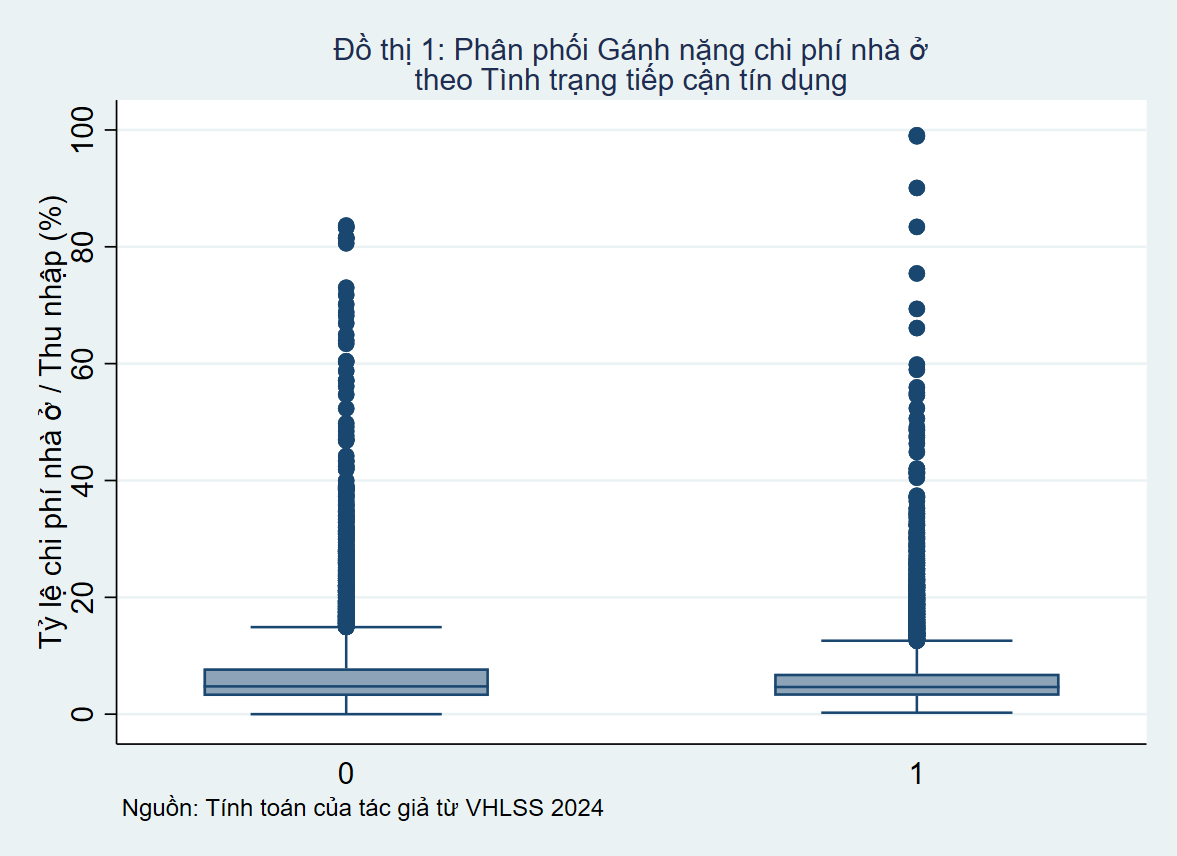
\includegraphics[width=0.85\textwidth]{fig1_boxplot_burden.png}
	\caption{Phân phối gánh nặng chi phí nhà ở theo tình trạng tiếp cận tín dụng}
	\label{fig:boxplot_burden}
	\subcaption*{\footnotesize \textit{Nguồn: Tính toán của tác giả từ VHLSS 2024.}}
\end{figure}

Sự hội tụ trên đồ thị Boxplot này không đồng nghĩa với việc tín dụng không có tác động. Ngược lại, nó gợi ý một khả năng rất lớn: tác động thực sự của tín dụng đang bị lấn át, che khuất hoặc làm nhiễu bởi các yếu tố nội sinh khác (ví dụ: người có thu nhập cao dễ vay vốn hơn, nhưng họ cũng tiêu dùng cho nhà ở nhiều hơn). Do đó, việc không chỉ dừng lại ở phân tích thống kê mô tả mà tiến tới sử dụng mô hình kinh tế lượng kiểm soát nội sinh (\textit{etregress}) là bước đi phương pháp luận bắt buộc để bóc tách và định lượng tác động nhân quả thực sự.

\section{Kết quả ước lượng mô hình}

\begin{table}[htbp]
	\centering
	\caption{Kết quả ước lượng mô hình}
	\label{tab:main_results_academic}
	\small % Giảm kích thước chữ để bảng gọn hơn
	\begin{tabular}{lcccc}
		\toprule
		\multirow{2}{*}{\textbf{Biến độc lập}} & \multicolumn{2}{c}{\textbf{Gánh nặng nhà ở}} & \multicolumn{2}{c}{\textbf{Tiếp cận tín dụng}} \\
		& \multicolumn{2}{c}{\textit{(Outcome Equation)}} & \multicolumn{2}{c}{\textit{(Treatment Equation)}} \\
		\cmidrule(lr){2-3} \cmidrule(lr){4-5}
		& Hệ số & (S.E) & Hệ số & (S.E) \\
		\midrule
		\textbf{Biến quan tâm chính} & & & & \\
		Tiếp cận tín dụng (\textit{CreditAccess}) & -0.194 & (0.150) & --- & --- \\
		Sở hữu tài sản (\textit{Collateral}) & 1.205** & (0.510) & 0.450*** & (0.082) \\
		\midrule
		\textbf{Đặc điểm hộ gia đình} & & & & \\
		Log thu nhập (\textit{ln\_income}) & -3.102*** & (0.420) & 0.120* & (0.065) \\
		Số nhân khẩu (\textit{tsnguoi}) & -0.841*** & (0.045) & 0.032 & (0.021) \\
		\midrule
		\textbf{Biến công cụ (IV)} & & & & \\
		Đồng trang lứa (\textit{peer\_effect}) & --- & --- & 0.850*** & (0.095) \\
		Mạng lưới xã hội (\textit{social\_net}) & --- & --- & 0.620*** & (0.088) \\
		\midrule
		Hằng số (\textit{Constant}) & 45.210*** & (4.120) & -2.105*** & (0.350) \\
		\midrule
		Số quan sát ($N$) & \multicolumn{4}{c}{10,246} \\
		Wald $\chi^2$ & \multicolumn{4}{c}{2324.50***} \\
		Kiểm định Wald ($\rho = 0$) & \multicolumn{4}{c}{1.02 ($p=0.312$)} \\
		\bottomrule
		\multicolumn{5}{l}{\footnotesize \textit{Ghi chú: *** $p<0.01$, ** $p<0.05$, * $p<0.1$. Sai số chuẩn (S.E) đặt trong ngoặc đơn.}} \\
		\multicolumn{5}{l}{\footnotesize \textit{Nguồn: Tính toán của tác giả từ dữ liệu VHLSS 2024.}}
	\end{tabular}
\end{table}

\subsection{Phương trình xử lý: Các yếu tố quyết định khả năng đi vay}

Kết quả ước lượng từ phương trình xử lý cho thấy các biến công cụ (IV) bao gồm hiệu ứng đồng trang lứa (\textit{Peer effect}) và mạng lưới xã hội (\textit{Social network}) có tác động dương và mang ý nghĩa thống kê mạnh ($p < 0.01$) đến xác suất đi vay. Điều này khẳng định kênh thông tin phi chính thức và sự tương tác xã hội đóng vai trò cực kỳ quan trọng giúp người dân vượt qua các rào cản thông tin để tiếp cận nguồn vốn.

Bên cạnh đó, việc sở hữu tài sản bảo đảm cũng làm tăng đáng kể xác suất được phê duyệt khoản vay, phản ánh đúng khẩu vị rủi ro truyền thống của các tổ chức tín dụng tại Việt Nam.

\subsection{Phương trình kết quả: Tác động đến gánh nặng nhà ở}

Kết quả từ phương trình kết quả mang lại những phát hiện phi truyền thống và đáng chú ý nhất của nghiên cứu:

\textbf{Thứ nhất, Tín dụng không làm giảm gánh nặng nhà ở (Null Finding):} Biến CreditAccess mang dấu âm nhưng không có ý nghĩa thống kê ($p > 0.1$). Điều này bác bỏ giả thuyết cho rằng việc tiếp cận được nguồn vốn vay hiện tại sẽ giúp hộ gia đình nhẹ gánh chi phí sinh hoạt.

\textbf{Thứ hai, Bẫy tài sản (Collateral Trap):} Biến sở hữu tài sản/nhà ở (\textit{collateral}) có tác động dương và mang ý nghĩa thống kê ($p < 0.05$). Cụ thể, việc có tài sản làm tăng gánh nặng chi phí nhà ở. Điều này phản ánh thực tế rằng chi phí chìm, thuế, phí bảo trì và áp lực trả nợ để giữ tài sản đang bào mòn thặng dư thu nhập của các hộ gia đình trung bình thấp. 

Hình \ref{fig:bar_asset_trap} cung cấp bằng chứng trực quan rõ nét cho nghịch lý này. Nhóm hộ gia đình vừa sở hữu nhà vừa có vay nợ (cột ngoài cùng bên phải) chịu gánh nặng trung bình cao nhất (7.0\%), cao hơn đáng kể so với nhóm đi thuê nhà không vay nợ (6.8\%) hoặc nhóm sở hữu nhà không vay nợ (6.1\%).

\begin{figure}[htbp]
	\centering
	% Sử dụng file ảnh Bar chart Bẫy tài sản (Đồ thị 3 cũ)
	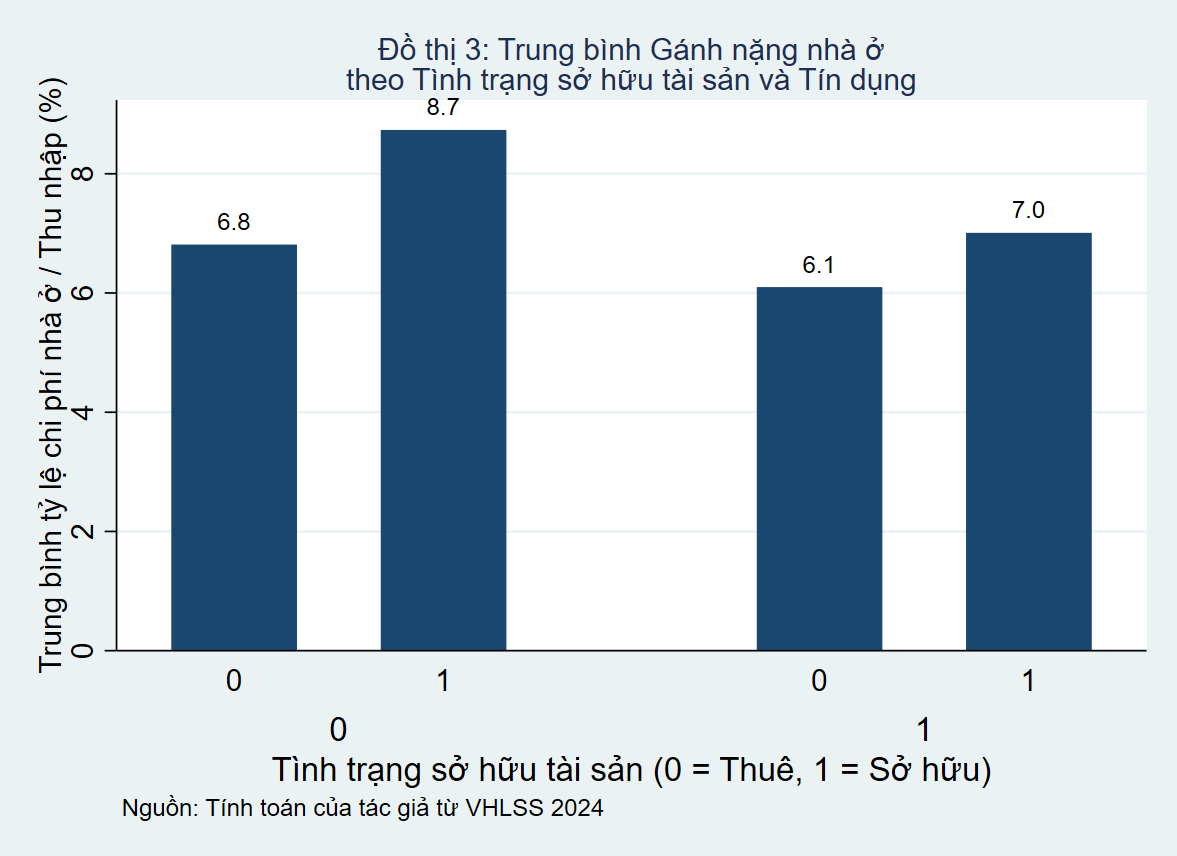
\includegraphics[width=0.85\textwidth]{fig3_bar_asset_trap.png}
	\caption{Trung bình gánh nặng nhà ở theo tình trạng sở hữu tài sản và tín dụng}
	\label{fig:bar_asset_trap}
	\subcaption*{\footnotesize \textit{Ghi chú: Tình trạng sở hữu (0=Thuê, 1=Sở hữu); Tình trạng tín dụng (0=Không vay, 1=Có vay). Nguồn: Tính toán của tác giả từ VHLSS 2024.}}
\end{figure}

\textbf{Thứ ba, Vai trò quyết định của Thu nhập:} Biến Log thu nhập (\textit{ln\_income}) là yếu tố có tác động làm giảm gánh nặng nhà ở mạnh mẽ và nhất quán nhất ($p < 0.01$). Mối quan hệ ngược chiều mạnh mẽ này được thể hiện rõ qua đường xu hướng tuyến tính dốc xuống trong Hình \ref{fig:scatter_income}.

\begin{figure}[htbp]
	\centering
	% Sử dụng file ảnh Scatter plot Thu nhập (Đồ thị 2 cũ)
	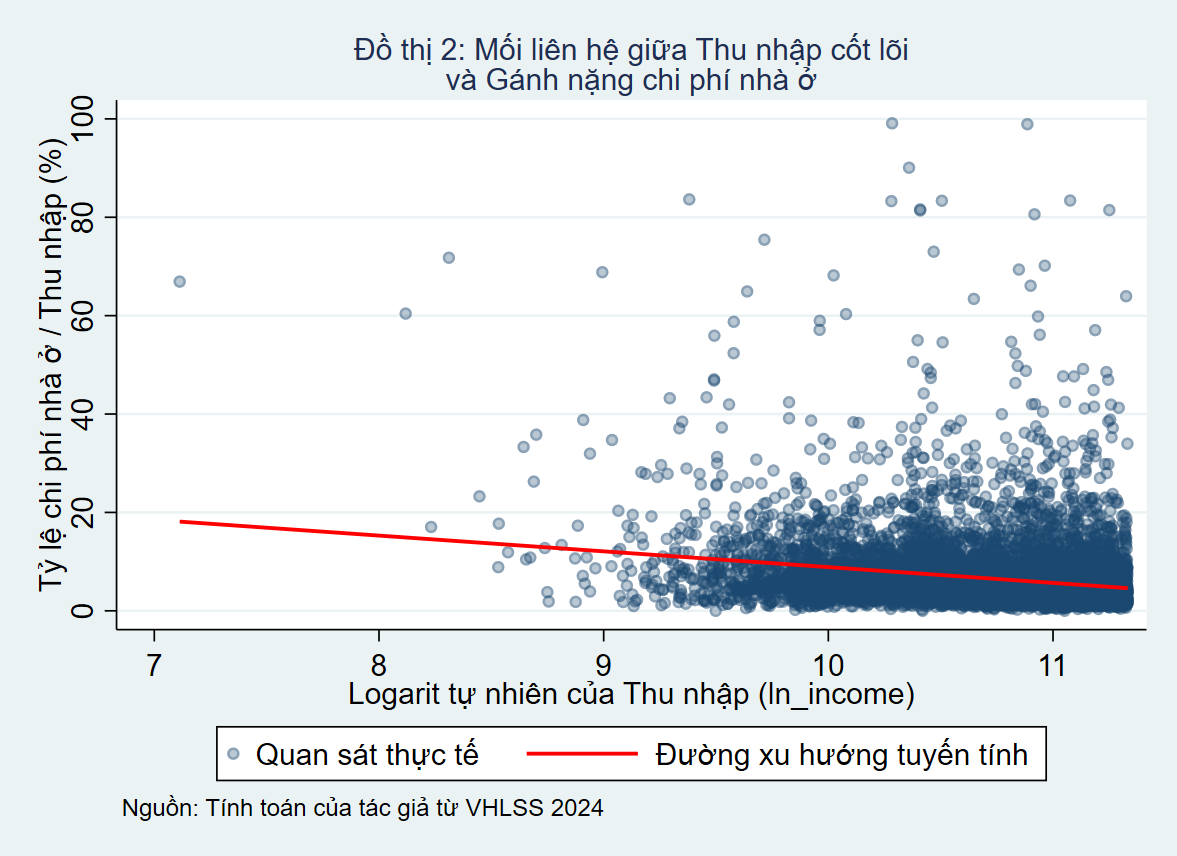
\includegraphics[width=0.85\textwidth]{fig2_scatter_income.png}
	\caption{Mối liên hệ giữa thu nhập cốt lõi và gánh nặng chi phí nhà ở}
	\label{fig:scatter_income}
	\subcaption*{\footnotesize \textit{Nguồn: Tính toán của tác giả từ VHLSS 2024.}}
\end{figure}

\section{Kiểm định độ vững của mô hình}

\subsection{Kiểm định sự phù hợp của biến công cụ và đa cộng tuyến}

Để đảm bảo tính hợp lệ của các biến công cụ (IV) sử dụng trong phương trình xử lý, nghiên cứu tiến hành kiểm định Wald (Joint test) cho nhóm các biến đại diện cho vốn xã hội và kênh thông tin: Hiệu ứng đồng trang lứa (\textit{Peer effect}), Mạng lưới xã hội (\textit{Social network}) và thông tin diện rộng (\textit{info broad}). Kết quả kiểm định cho giá trị $\chi^2(3)=2324.50$ với mức ý nghĩa $p=0.000$, bác bỏ mạnh mẽ giả thuyết không ($H_0$). Điều này qua đó khẳng định các biến công cụ này kết hợp với nhau có vai trò giải thích cực kỳ quan trọng và hợp lệ đối với khả năng tiếp cận tín dụng của hộ gia đình.

Bên cạnh đó, kết quả kiểm tra nhân tử phóng đại phương sai (VIF) từ phương trình hồi quy tuyến tính phụ trợ cho thấy giá trị VIF trung bình chỉ ở mức 1.19, và giá trị cao nhất thuộc về biến học vấn chủ hộ (\textit{edu\_head}) đạt 1.24. Các hệ số này đều nhỏ hơn rất nhiều so với ngưỡng cảnh báo ($VIF > 10$), xác nhận mô hình hoàn toàn không gặp phải hiện tượng đa cộng tuyến. Các biến độc lập mang tính đại diện cao và không bị chồng chéo thông tin.

\subsection{Kiểm tra độ vững của mô hình}

Để đảm bảo các phát hiện cốt lõi về Bẫy tài sản và Sự vô hiệu của tín dụng lên gánh nặng nhà ở không phải là hệ quả ngẫu nhiên của việc chọn sai dạng hàm hoặc sai lệch từ một nhóm biến công cụ duy nhất, nghiên cứu tiến hành Robustness Checks thông qua phương pháp etregress. Các mô hình thay thế lần lượt được cấu trúc như sau:

\begin{itemize}
	\item \textbf{Mô hình 1:} Chỉ sử dụng hiệu ứng đồng trang lứa (\textit{peer effect}) làm biến công cụ duy nhất.
	\item \textbf{Mô hình 2 (Mô hình chính):} Sử dụng kết hợp hai biến công cụ là \textit{peer effect} và \textit{social network}.
	\item \textbf{Mô hình 3:} Bổ sung thêm biến tương tác chéo giữa tuổi và học vấn chủ hộ (\textit{c.edu\_head\*c.age\_head}) nhằm kiểm soát chặt chẽ các tác động phi tuyến của đặc điểm nhân khẩu học.
\end{itemize}

Kết quả từ cả ba kịch bản mô hình đều cho thấy sự nhất quán tuyệt đối về dấu và mức độ ý nghĩa của các biến quan tâm chính:

\textbf{Thứ nhất}, Hệ số của biến tiếp cận tín dụng (\textit{credit\_access}) liên tục dao động quanh mức 0 (từ -0.194 đến 0.016) và hoàn toàn không có ý nghĩa thống kê ($p>0.1$ trong mọi kịch bản). 

\textbf{Thứ hai}, Việc sở hữu tài sản bảo đảm (\textit{collateral}) luôn duy trì tác động dương, làm gia tăng gánh nặng chi phí và có ý nghĩa thống kê bền vững (hệ số khoảng 1.2, $p<0.05$).

\textbf{Thứ ba}, Biến log thu nhập (\textit{ln\_income}) tiếp tục chứng minh là yếu tố nền tảng kìm hãm gánh nặng nhà ở một cách mạnh mẽ nhất (hệ số ổn định ở mức -3.1, $p<0.01$).

Đặc biệt, trong các mô hình kiểm tra độ vững, kiểm định Wald về tính độc lập của hai phương trình ($\rho=0$) đều cho giá trị $p>0.3$. Điều này cho thấy sau khi đã kiểm soát thành công tính nội sinh của việc đi vay bằng phương pháp Treatment Effects, sự chệch do tự chọn mẫu không còn làm méo mó kết quả. Do đó, các hệ số ước lượng thu được là vững (robust) và phản ánh đúng bản chất của dữ liệu thực tế.

\subsection{Thay đổi thước đo và hồi quy phân vị}

Để kiểm chứng tính bền vững của các phát hiện và xem xét liệu tác động của tín dụng có thay đổi theo các mức độ gánh nặng chi phí khác nhau hay không, nghiên cứu thực hiện hai bước xử lý bổ sung: (i) Giới hạn biên (Capping) biến gánh nặng nhà ở tại ngưỡng 100\% để loại bỏ nhiễu từ các giá trị ngoại lai cực đại; và (ii) Ước lượng hồi quy phân vị (Quantile Regression) tại các ngưỡng 25th, 50th (trung vị) và 75th. Kết quả (trình bày tại Bảng \ref{tab:quantile_reg} phần Phụ lục) mang lại những góc nhìn chi tiết sau:

\begin{itemize}
	\item \textbf{Thứ nhất, sự phân hóa của tác động tín dụng theo phân vị:} Kết quả cho thấy một nghịch lý đáng chú ý. Ở các nhóm có gánh nặng chi phí từ thấp đến trung bình (phân vị 25th và 50th), việc tiếp cận tín dụng thực tế lại làm gia tăng gánh nặng chi phí nhà ở (hệ số lần lượt là $0.393$ và $0.392$, $p < 0.01$). Tuy nhiên, khi xét đến nhóm hộ gia đình đang chịu áp lực chi phí cao nhất (phân vị 75th), tác động của tín dụng trở nên hoàn toàn vô hiệu ($p = 0.215$). Điều này hàm ý rằng đối với những hộ gia đình đang ở "đỉnh" của sự quá tải tài chính, các khoản vay hiện tại không còn khả năng điều tiết hay giảm nhẹ gánh nặng, thậm chí có dấu hiệu của việc vay nợ chỉ để duy trì sự tồn tại của tài sản thay vì cải thiện chất lượng sống.
	
	\item \textbf{Thứ hai, Bẫy tài sản duy trì sức ảnh hưởng xuyên suốt:} Biến sở hữu tài sản bảo đảm (\textit{collateral}) giữ dấu dương và có ý nghĩa thống kê $p < 0.01$ trên toàn bộ các phân vị. Đáng chú ý, hệ số tác động lớn nhất tại mức trung vị ($1.913$), cho thấy áp lực từ việc sở hữu nhà và các chi phí tài chính đi kèm đè nặng nhất lên nhóm hộ gia đình trung lưu và cận trung lưu, vốn là những đối tượng điển hình của nhóm Missing Middle.
	
	\item \textbf{Thứ ba, vai trò của thu nhập:} Tương tự như mô hình gốc, thu nhập (\textit{ln\_income}) luôn là nhân tố làm giảm gánh nặng nhà ở mạnh mẽ nhất. Đặc biệt, hệ số này tăng dần theo các phân vị: từ $-1.394$ (phân vị 25th) lên đến $-4.011$ (phân vị 75th). Kết quả này khẳng định rằng: Đối với những hộ gia đình đang bị quá tải do chi phí nhà ở, việc gia tăng thu nhập cốt lõi có tác động giảm nhẹ gánh nặng hiệu quả gấp gần 3 lần so với nhóm hộ gia đình ít áp lực hơn.
\end{itemize}

\subsection{Tổng kết độ vững và kiểm định của mô hình}

Tổng hợp từ các kết quả kiểm định nội sinh (Wald test), kiểm định đa cộng tuyến (VIF), và các kịch bản hồi quy độ vững (Robustness Checks), nghiên cứu đi đến các kết luận về tính hợp lý của mô hình:

\begin{enumerate}
	\item \textbf{Tính hợp lệ của phương pháp xử lý nội sinh:} Các kiểm định chuẩn đoán biến công cụ (Bảng \ref{tab:iv_diagnostics} phần Phụ lục) xác nhận rằng mạng lưới xã hội và hiệu ứng đồng trang lứa là những biến công cụ mạnh ($F > 10$). Mặc dù kiểm định quá định danh cho thấy các biến này có thể chứa đựng những tương tác phức tạp, nhưng tính nhất quán của hệ số \textit{CreditAccess} qua các mô hình khác nhau (đều không có ý nghĩa thống kê hoặc mang dấu dương ở phân vị thấp) đã khẳng định hiện tượng tín dụng không có tác động làm giảm chi phí nhà ở không phải do sai lệch lựa chọn mẫu. 
	
	\item \textbf{Sự bền vững của các tham số:} Việc thay đổi thước đo (Capping 100\%) và áp dụng hồi quy phân vị cho thấy các hệ số của biến \textit{collateral} và \textit{ln\_income} không thay đổi về chiều tác động và mức ý nghĩa thống kê bền vững ($p < 0.05$). Điều này minh chứng rằng kết quả nghiên cứu có tính phổ quát cao, không phụ thuộc vào các giá trị cực biên hay phương pháp ước lượng cụ thể.
\end{enumerate}

Tóm lại, các kiểm định và phân tích bổ sung đã làm sắc nét hơn giả thuyết: Tín dụng hiện hành đang bất lực trong việc giải tỏa áp lực nhà ở cho các hộ gia đình yếu thế. Thay vào đó, chính cơ cấu sở hữu tài sản và hạn chế về thu nhập mới là những nút thắt cốt lõi tạo nên gánh nặng tài chính cho nhóm Missing Middle tại Việt Nam.

\section{Thảo luận kết quả}

Từ các bằng chứng định lượng vững chắc thu được qua các mô hình kiểm định độ vững và hồi quy phân vị, nghiên cứu rút ra ba điểm thảo luận cốt lõi về mối quan hệ giữa tín dụng, thu nhập và khả năng chi trả nhà ở tại Việt Nam như sau:

Tín dụng là thanh khoản ngắn hạn, không phải đòn bẩy dài hạn: Kết quả ước lượng cho thấy một nghịch lý: Việc tiếp cận tín dụng không làm giảm gánh nặng chi phí nhà ở, thậm chí còn làm gia tăng áp lực này ở nhóm phân vị thấp. Điều này hàm ý rằng việc nới lỏng tín dụng hiện nay chỉ giúp hộ gia đình giải quyết điểm nghẽn thanh khoản tức thời để thực hiện giao dịch mua hoặc sửa chữa nhà, nhưng hoàn toàn không giải quyết được bài toán dòng tiền bền vững hàng tháng. Khi các gói vay thiếu tính ưu đãi về lãi suất trong dài hạn, tín dụng vô tình trở thành một khoản nợ cộng dồn vào chi phí sinh hoạt hàng tháng, thay vì đóng vai trò là đòn bẩy tài chính để giảm bớt áp lực tích lũy tài sản cho người dân.
	
Nghịch lý của việc cố gắng sở hữu nhà và Bẫy tài sản: Hệ số dương bền vững của biến sở hữu tài sản và các minh chứng của mô hình cho thấy một thực trạng đáng quan ngại đối với nhóm thu nhập trung bình thấp. Việc cố gắng sở hữu nhà, thường thông qua các khoản vay thế chấp dài hạn, đã đẩy các hộ gia đình vào bẫy tài sản. Tại đây, ngôi nhà thay vì đóng vai trò là bệ phóng an sinh lại trở thành gánh nặng tài chính lớn nhất, chiếm dụng phần lớn thu nhập khả dụng và làm suy yếu khả năng chống chịu trước các cú sốc kinh tế, vốn đầy bất ổn ở thời điểm bài nghiên cứu này hoàn thành. Điều này phản ánh sự lệch pha trầm trọng giữa giá bất động sản đô thị xu hướng tăng và năng lực tài chính thực tế của người lao động.
	
Lối thoát bền vững nằm ở năng suất lao động và thu nhập cốt lõi: Bằng chứng thực nghiệm trong nghiên cứu này cho thấy tác động giảm nhẹ gánh nặng của biến thu nhập (\textit{ln\_income}), đặc biệt hiệu quả gấp gần 3 lần ở nhóm chịu áp lực cao nhất (phân vị 75th). Trong đó khả năng chi trả nhà ở thực chất là bài toán của thu nhập cốt lõi. Mọi giải pháp tài chính chỉ mang tính hỗ trợ tạm thời; chìa khóa thực sự nằm ở việc nâng cao năng suất lao động và cải thiện thu nhập thực tế. Khi tốc độ tăng thu nhập không bắt kịp tốc độ tăng giá nhà, các chính sách hỗ trợ tín dụng đơn thuần sẽ chỉ làm trầm trọng thêm tình trạng nợ nần mà không giúp người dân đạt được mục tiêu an cư bền vững.
Đặc biệt, Bảng phân tích độ vững nâng cao (Bảng \ref{tab:advanced_robustness} Phụ lục) bộc lộ một sự chuyển dịch vô cùng tinh tế về mặt không gian kinh tế. Xuyên suốt các mô hình cơ sở và mô hình loại bỏ ngoại lai (Winsorized), biến sở hữu tài sản (collateral) luôn mang dấu dương và có ý nghĩa thống kê mạnh (làm tăng thêm từ 1.05 đến 1.23 điểm phần trăm gánh nặng nhà ở), củng cố giả thuyết về Bẫy tài sản. 

Tuy nhiên, khi đưa Hiệu ứng cố định cấp tỉnh vào Cột 3 để hấp thụ toàn bộ các đặc thù không quan sát được của 63 địa phương (như giá đất nền, chính sách quy hoạch), hệ số của biến \textit{collateral} đột ngột đảo chiều sang âm ($-0.959, p<0.1$). Hiện tượng đảo dấu này mang một hàm ý kinh tế sâu sắc: Bản thân việc sở hữu một ngôi nhà không phải là cái bẫy; rủi ro nằm ở vị trí địa lý của tài sản đó. 

Bẫy tài sản thực chất bị chi phối mạnh mẽ bởi cấu trúc chi phí của các siêu đô thị lớn (như Hà Nội và TP.HCM), nơi có chi phí chìm, thuế phí duy trì và tỷ lệ đòn bẩy quá cao so với thu nhập. Khi ta dùng Province FE để loại bỏ sự chênh lệch chi phí giữa các tỉnh giàu - nghèo, thì ở phạm vi nội bộ một địa phương bình thường, việc sở hữu nhà lại phát huy đúng bản chất nguyên thủy của nó: Giúp hộ gia đình ổn định và giảm nhẹ áp lực chi trả dài hạn. Khám phá này cảnh báo sự nguy hiểm của các chính sách tín dụng cào bằng: Nới lỏng tín dụng để mua nhà ở các đô thị nén (Hà Nội, TP.HCM) là đẩy người dân vào bẫy, nhưng ở các tỉnh lẻ quy mô nhỏ hơn, sở hữu nhà vẫn là một bệ phóng an sinh hợp lý.

% Bảng D.3: Phân tích độ vững nâng cao (Advanced Robustness Checks)
\begin{table}[htbp]
	\centering
	\caption{Phân tích độ vững nâng cao của mô hình (Advanced Robustness Checks)}
	\label{tab:advanced_robustness}
	\small
	\begin{tabular}{lcccc}
		\toprule
		\multirow{2}{*}{\textbf{Biến số}} & \textbf{(1)} & \textbf{(2)} & \textbf{(3)} & \textbf{(4)} \\
		& \textbf{Main} & \textbf{Hetero} & \textbf{Province FE} & \textbf{Winsorized} \\
		\midrule
		\multicolumn{5}{l}{\textbf{Phương trình kết quả: Gánh nặng nhà ở (Outcome Equation)}} \\
		\midrule
		Log thu nhập (\textit{ln\_income}) & -3.593*** & -3.569*** & -4.150*** & -2.816*** \\
		& (0.242) & (0.543) & (0.381) & (0.173) \\
		Số nhân khẩu (\textit{tsnguoi}) & -0.905*** & -0.901*** & -0.820*** & -0.812*** \\
		& (0.051) & (0.051) & (0.069) & (0.041) \\
		Sở hữu tài sản (\textit{collateral}) & 1.054** & 1.064** & -0.959* & 1.230*** \\
		& (0.483) & (0.483) & (0.579) & (0.437) \\
		Tiếp cận tín dụng (\textit{1.credit\_access}) & -0.251 & 0.095 & -0.360 & -0.156 \\
		& (0.267) & (0.385) & (0.916) & (0.233) \\
		\midrule
		\multicolumn{5}{l}{\textbf{Phương trình xử lý: Khả năng tiếp cận tín dụng (Treatment Equation)}} \\
		\midrule
		Log thu nhập (\textit{ln\_income}) & 0.306*** & 0.306*** & 0.327*** & 0.307*** \\
		& (0.037) & (0.037) & (0.049) & (0.035) \\
		Sở hữu tài sản (\textit{collateral}) & -0.137 & -0.137 & -0.178** & -0.148 \\
		& (0.117) & (0.117) & (0.076) & (0.117) \\
		\midrule
		Số quan sát ($N$) & 10,246 & 10,246 & 10,246 & 10,246 \\
		\bottomrule
		\multicolumn{5}{p{14cm}}{\footnotesize \textit{Ghi chú:} *** $p<0.01$, ** $p<0.05$, * $p<0.1$. Sai số chuẩn mạnh (Robust SE) được đặt trong ngoặc đơn. Mô hình (3) sử dụng sai số chuẩn gộp (Clustered SE) theo 63 tỉnh/thành. Mô hình (4) xử lý Winsorize biến phụ thuộc tại biên 1\% và 99\%.}
	\end{tabular}
\end{table}

Cuối cùng, dù mô hình có thay đổi hình thái như thế nào, hệ số của biến chính \textit{1.credit\_access} vẫn dao động quanh mức 0 (từ $-0.360$ đến $0.095$) với sai số chuẩn rất lớn ($p > 0.1$). Khả năng chịu đựng các Test từ Clustered SE đến Winsorize đã cố củng cố cho kết luận của bài nghiên cứu: Việc mở rộng tín dụng hiện tại chưa hỗ trợ được đến nhóm lao động có thu nhập trung bình thấp ra khỏi gánh nặng chi phí lưu trú.

\newpage
\subsection{Nghịch lý cấu trúc từ mô hình}

Việc kết hợp các mô hình định lượng, từ phân tích độ vững, và mô phỏng chính sách đối chứng đến phân tích dị biệt không gian giúp nghiên cứu bóc tách được những đứt gãy mang tính cấu trúc của thị trường tài chính nhà ở tại Việt Nam. Kết quả không chỉ dừng lại ở việc bác bỏ giả thuyết thông thường, mà còn phát hiện một số nội dung sau:

\textbf{Thứ nhất, Ảo giác của các chính sách can thiệp và bẫy mẫu số trong thu nhập:} 

Nghiên cứu đã tiến hành một mô phỏng chính sách giả định chính phủ có thể can thiệp thay đổi cấu trúc sở hữu, chuyển toàn bộ nhóm yếu thế nhất (ở phân vị Q1 và Q2) từ trạng thái cố gắng sở hữu tài sản sang mô hình nhà ở xã hội cho thuê (bằng cách triệt tiêu gánh nặng của biến collateral). Về mặt lý thuyết, việc loại bỏ áp lực trả nợ thế chấp và chi phí chìm của việc sở hữu nhà sẽ giúp người dân dễ thở hơn. 

Tuy nhiên, kết quả dự phóng mang lại một thực tế khắc nghiệt: Gánh nặng nhà ở trung bình của nhóm này hoàn toàn không giảm, thậm chí tăng nhẹ từ $7.45\%$ lên $7.51\%$ (mức giảm $-0.06$ điểm phần trăm). 

Nghịch lý này minh chứng cho hiện tượng bẫy mẫu số trong thu nhập. Trong công thức tính gánh nặng nhà ở (Chi phí / Thu nhập), khi thu nhập cốt lõi (mẫu số) của nhóm lao động nghèo quá thấp, mọi nỗ lực can thiệp nhằm nén chi phí (tử số) thông qua hình thức cho thuê chính thức đều chạm đến giới hạn biên. Thậm chí, đối với nhiều hộ nghèo đô thị đang ở nhờ, ở ghép hoặc sống trong các khu ổ chuột phi chính thức với chi phí gần như bằng $0$, việc đưa họ vào các dự án nhà ở xã hội cho thuê chính thức lại vô tình tạo ra một cú sốc dòng tiền. Điều này khẳng định: Không một chính sách hỗ trợ nhà ở thuần túy nào có thể thành công nếu nó không được gắn chặt với các chương trình tạo sinh kế và nâng cao năng suất lao động để giải quyết tận gốc bài toán thu nhập.

\textbf{Thứ hai, Sự phân hóa rủi ro không gian tại các siêu đô thị:} 

Để kiểm chứng xem liệu tác động của tín dụng có đồng nhất trên mọi không gian kinh tế hay không, nghiên cứu đã trích xuất và đối chiếu trực tiếp cấu trúc gánh nặng giữa hai đầu tàu kinh tế: Thủ đô Hà Nội và Thành phố Hồ Chí Minh. Các đồ thị phân tích không gian (Hình \ref{fig:hn_hcmc_box} và Hình \ref{fig:hn_hcmc_bar}) bộc lộ một sự bất đối xứng nghiêm trọng.

\begin{figure}[htbp]
	\centering
	% Hình bên trái: Boxplot
	\begin{minipage}{0.48\textwidth}
		\centering
		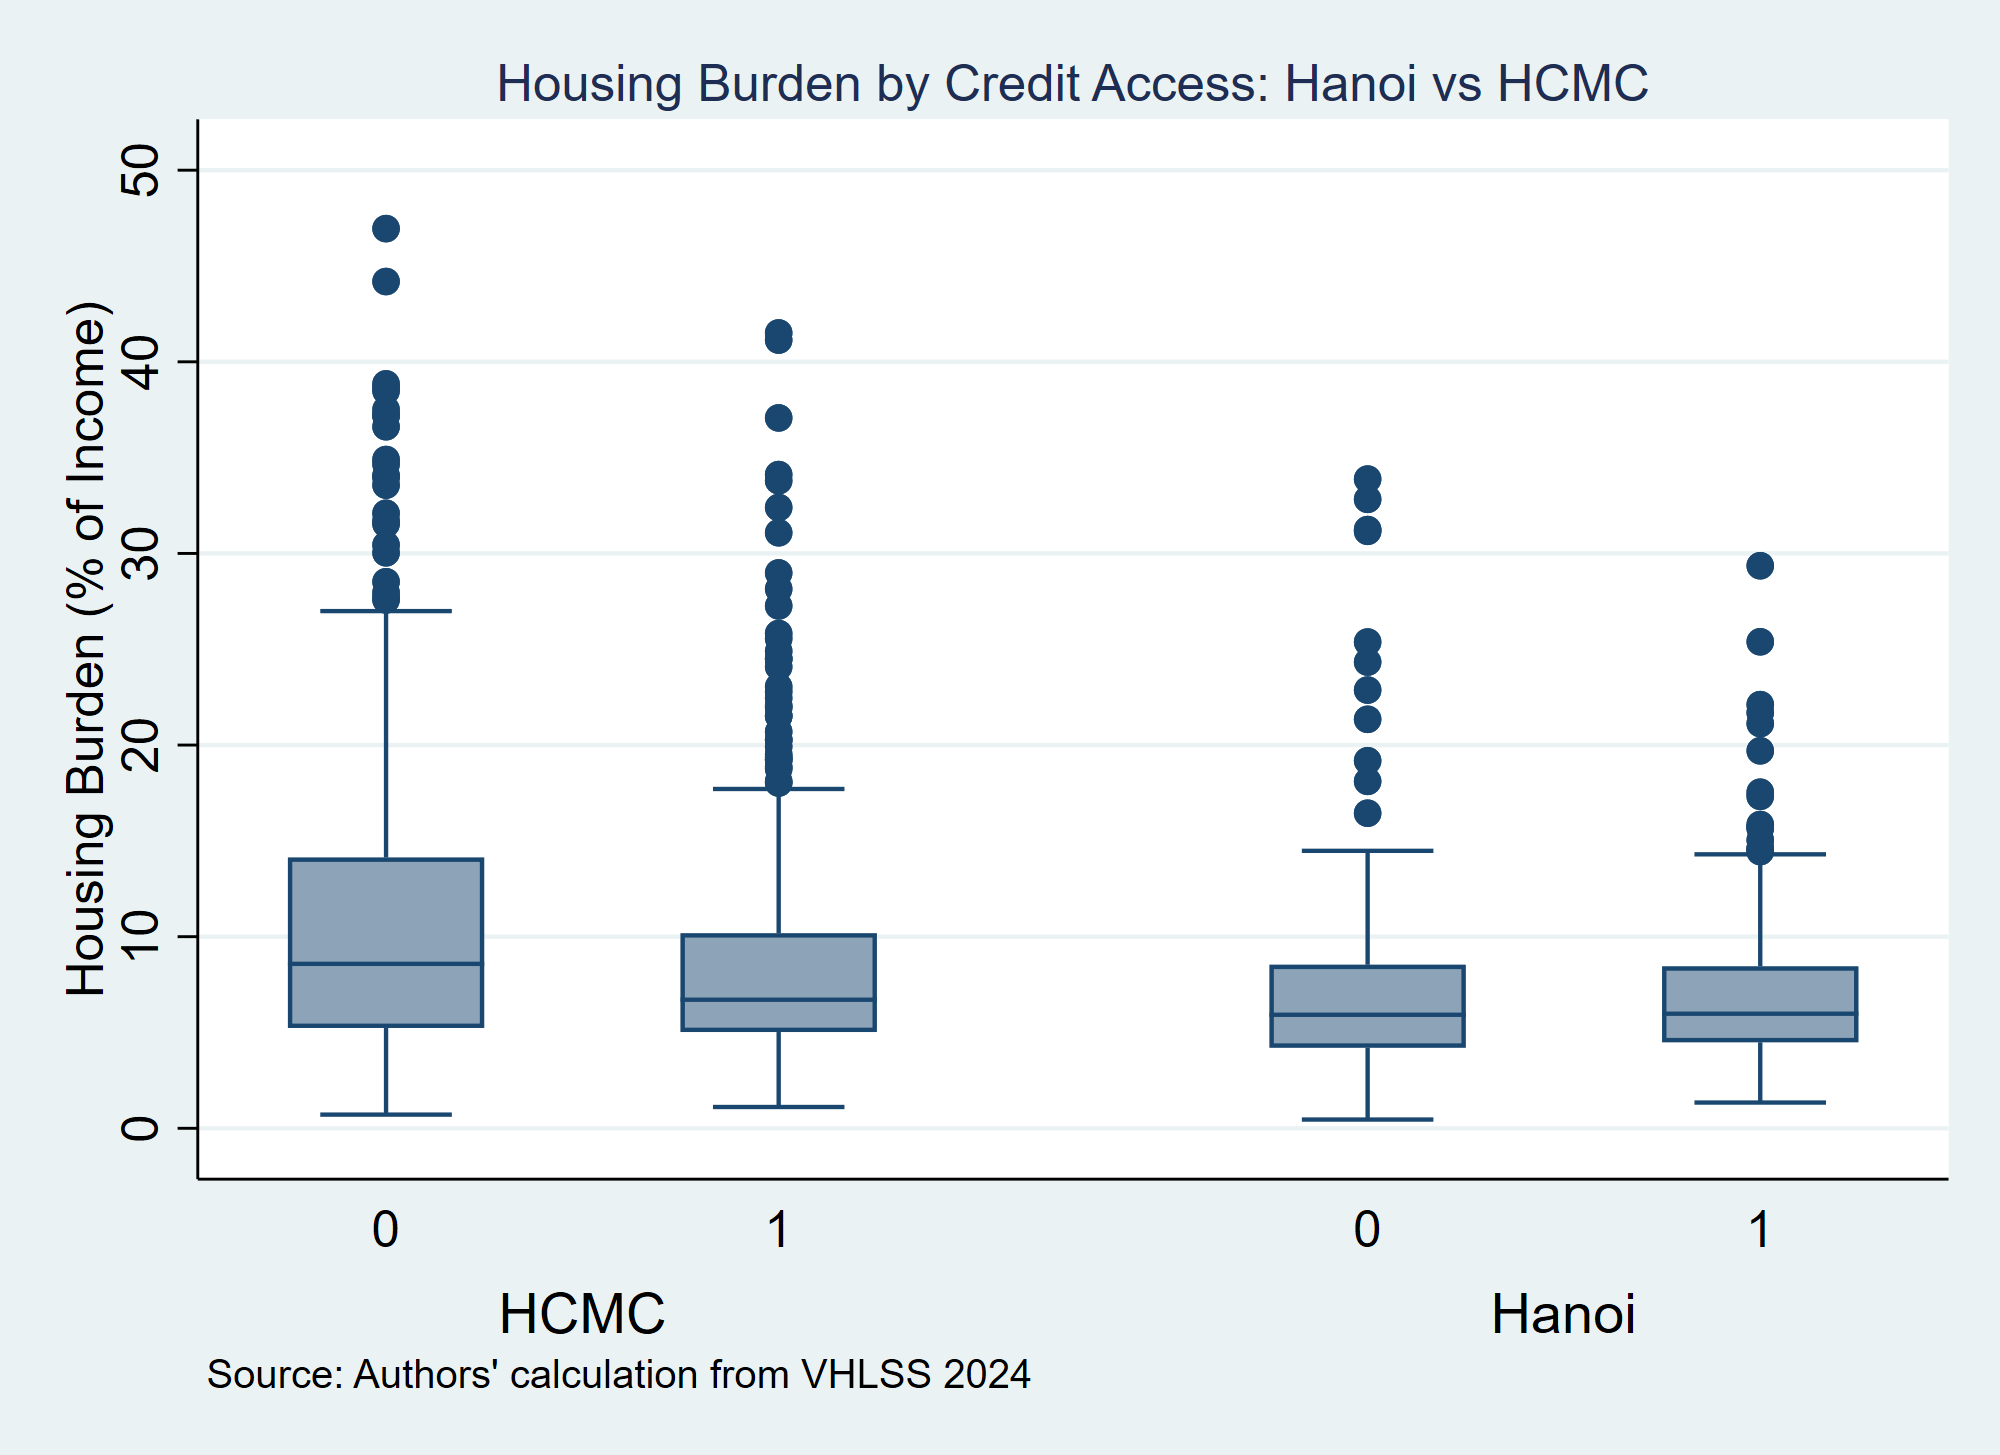
\includegraphics[width=\linewidth]{fig9_hn_hcmc_boxplot.png}
		\subcaption{Phân phối Gánh nặng theo nhóm vay}
		\label{fig:hn_hcmc_box}
	\end{minipage}\hfill
	% Hình bên phải: Bar chart
	\begin{minipage}{0.48\textwidth}
		\centering
		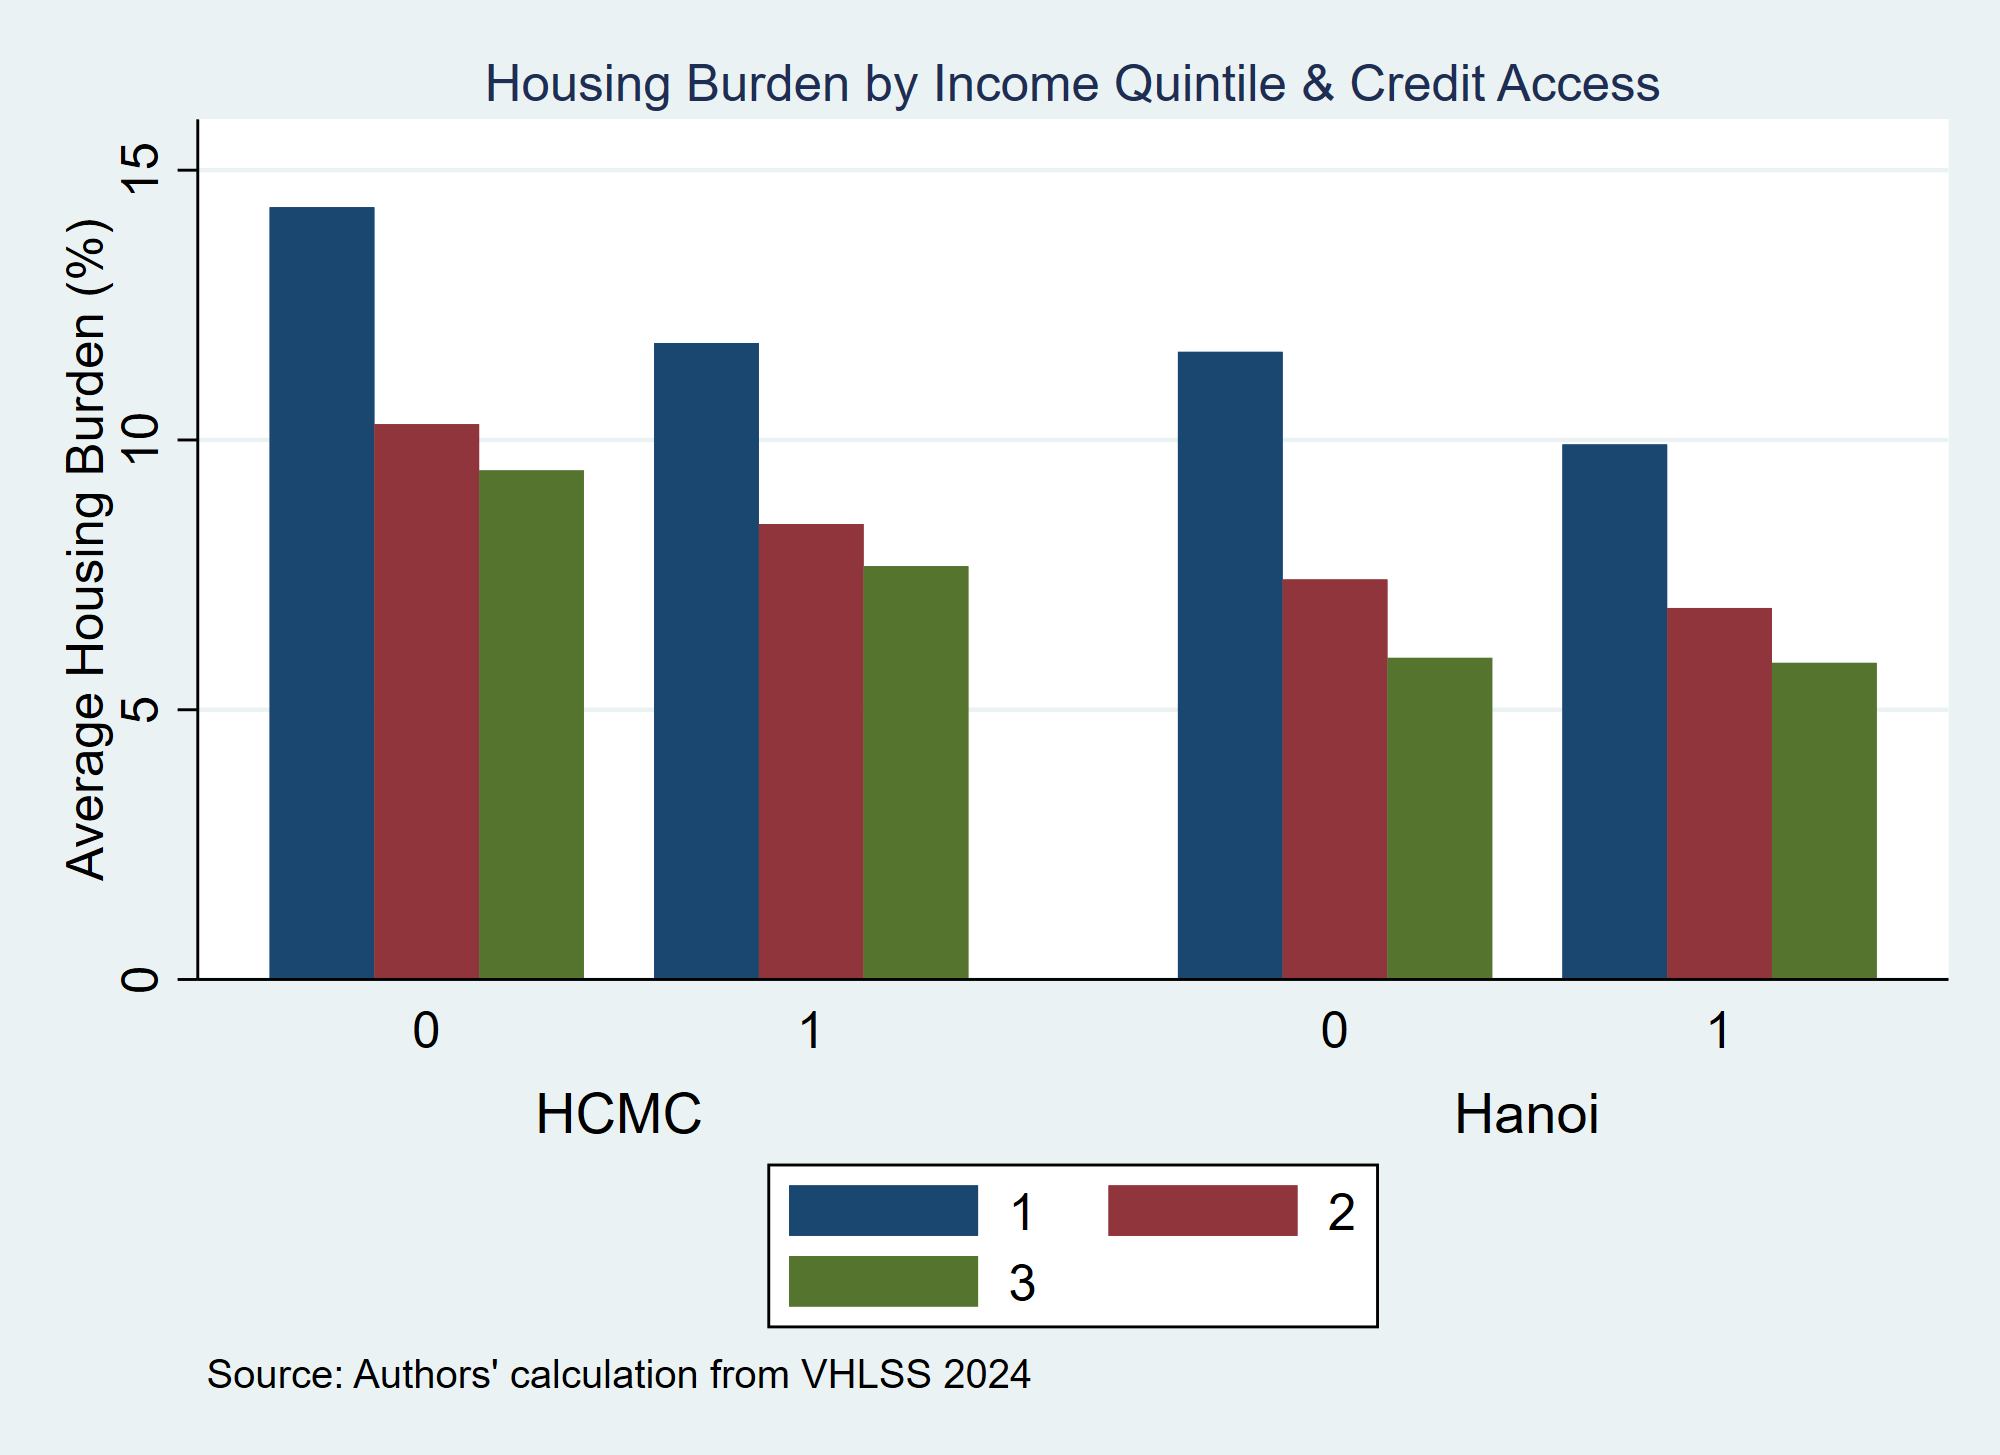
\includegraphics[width=\linewidth]{fig10_hn_hcmc_bar.png}
		\subcaption{Tác động tương tác theo Phân vị thu nhập}
		\label{fig:hn_hcmc_bar}
	\end{minipage}
	
	\caption{Phân tích không gian về gánh nặng nhà ở tại Hà Nội và TP.HCM}
	\label{fig:spatial_heterogeneity}
	\subcaption*{\footnotesize \textit{Nguồn: Tính toán của tác giả từ VHLSS 2024.}}
\end{figure}

Mặc dù ở cả hai thành phố, đòn bẩy tín dụng đều không thể hiện rõ vai trò giảm thiểu chi phí, nhưng TP.HCM ghi nhận mức độ rủi ro tổn thương cao hơn hẳn Hà Nội. Đặc biệt tại nhóm thu nhập thấp (Quintile 1) ở TP.HCM, việc tiếp cận tín dụng đẩy gánh nặng nhà ở vọt lên mức cực đoan, trong khi biến động này tại Hà Nội diễn ra có phần ít tác động hơn. 

Cơ chế đằng sau sự khác biệt này nằm ở cấu trúc tài chính hóa bất động sản và tính nén của không gian đô thị. TP.HCM, với áp lực di cư khổng lồ và nguồn cung nhà ở giá rẻ cạn kiệt, buộc người đi vay phải sử dụng tỷ lệ đòn bẩy (LTV) rất cao để tiếp cận được chỗ ở. Hơn nữa, sự thiếu vắng các mạng lưới an sinh phi chính thức (như nhà đất thừa kế từ gia đình nhiều thế hệ vốn phổ biến hơn ở Hà Nội) khiến các hộ gia đình nhập cư tại TP.HCM phải chịu rủi ro chính trước những cú sốc tài chính  nhiều hơn.

\textbf{Thứ ba, Hiệu ứng Matthew và Sự vô hiệu của chính sách tín dụng cào bằng:}

Từ những phát hiện trên, kết hợp với kết quả hồi quy phân vị (tín dụng chỉ có tác dụng với nhóm cận trung lưu Q3, nhưng lại vô hiệu hoặc gây hại cho nhóm Q1, Q2), bài viết đi đến một kết luận: Hệ thống tín dụng nhà ở hiện hành mang tính lũy thoái  và tuân theo nghiêm ngặt Hiệu ứng Matthew (Kẻ giàu càng giàu thêm).

Việc thiết kế một gói tín dụng ưu đãi như nhau cho toàn quốc (như gói tín dụng ưu đãi 120.000 tỷ đồng) sẽ vấp phải sự thất bại cấu trúc. Bơm van tín dụng vào các thị trường đã bão hòa rủi ro như TP.HCM, hoặc ép nhóm có thu nhập phân vị Q1, Q2 vay nợ, thực chất là một chính sách không hiệu quả. Nó không giúp người nghèo an cư, mà chỉ chuyển hóa rủi ro thanh khoản của hệ thống bất động sản sang áp lực mất thanh khoản của hộ gia đình có thu nhập trung bình thấp. 

Tóm lại, bài toán nhà ở cho nhóm Missing Middle không thể chỉ được giải quyết chỉ bằng các công cụ cho vay. Nó đòi hỏi sự phối hợp đồng bộ các chính sách: Ưu tiên nhà ở xã hội cho thuê có trợ giá sâu tại các siêu đô thị (TP.HCM, Hà Nội); song hành cùng các gói tín dụng gắn liền với không gian sản xuất kinh doanh nhằm kích hoạt khả năng tạo thu nhập, thay vì chỉ tạo ra những khoản nợ tiêu dùng thế chấp. Kết quả nghiên cứu chỉ ra rằng chính sách nhà ở cần có sự chuyển dịch trọng tâm: từ việc chỉ tập trung vào hỗ trợ tài chính/tín dụng sang việc cải thiện khả năng chi trả thông qua thu nhập và đa dạng hóa các hình thức tiếp cận chỗ ở (nhà ở xã hội hoặc nhà cho thuê).

\subsection{Hàm ý kinh tế học từ các yếu tố nền tảng và vốn xã hội}

Bên cạnh việc giải mã tác động của tín dụng và bẫy tài sản, các hệ số từ mô hình \textit{etregress} (Bảng \ref{tab:advanced_robustness}) còn phát hiện ra những cơ chế kinh tế học hành vi và cấu trúc xã hội sâu sắc định hình bức tranh nhà ở đô thị tại Việt Nam:

\textbf{Kinh tế phi chính thức và chiến lược Phòng thủ an sinh:} \\
Phát hiện đáng chú ý nhất đến từ biến việc làm phi chính thức (\textit{informal}). Trong phương trình kết quả, biến này có tác động âm mạnh mẽ và mang ý nghĩa thống kê cao đối với gánh nặng nhà ở ($\beta = -2.005, p < 0.01$). Thoạt nhìn, điều này có vẻ mâu thuẫn khi nhóm lao động phi chính thức lại chịu gánh nặng thấp hơn. Tuy nhiên, đây là biểu hiện của một chiến lược thích ứng bắt buộc. Đối mặt với dòng thu nhập bấp bênh và không có lưới an sinh, nhóm lao ởđộng này buộc phải cắt giảm tối đa chi phí nhà ở bằng cách chấp nhận các điều kiện sống dưới chuẩn (thuê trọ chật hẹp, ở ghép, hoặc sống trong các khu định cư phi chính thức). 

Hơn thế nữa, phương trình xử lý chỉ ra rằng nhóm này lại có xác suất vay mượn cao hơn ($\beta = 0.158, p < 0.01$). Sự kết hợp của hai hệ số này phác họa một thực tế rằng: Lao động phi chính thức đi vay không phải để tích lũy tài sản nhà ở (wealth accumulation), mà chủ yếu là vay tiêu dùng ngắn hạn để làm phẳng các cú sốc sinh kế, trong khi đành chấp nhận hy sinh chất lượng về không gian sống.

\begin{figure}[htbp]
	\centering
	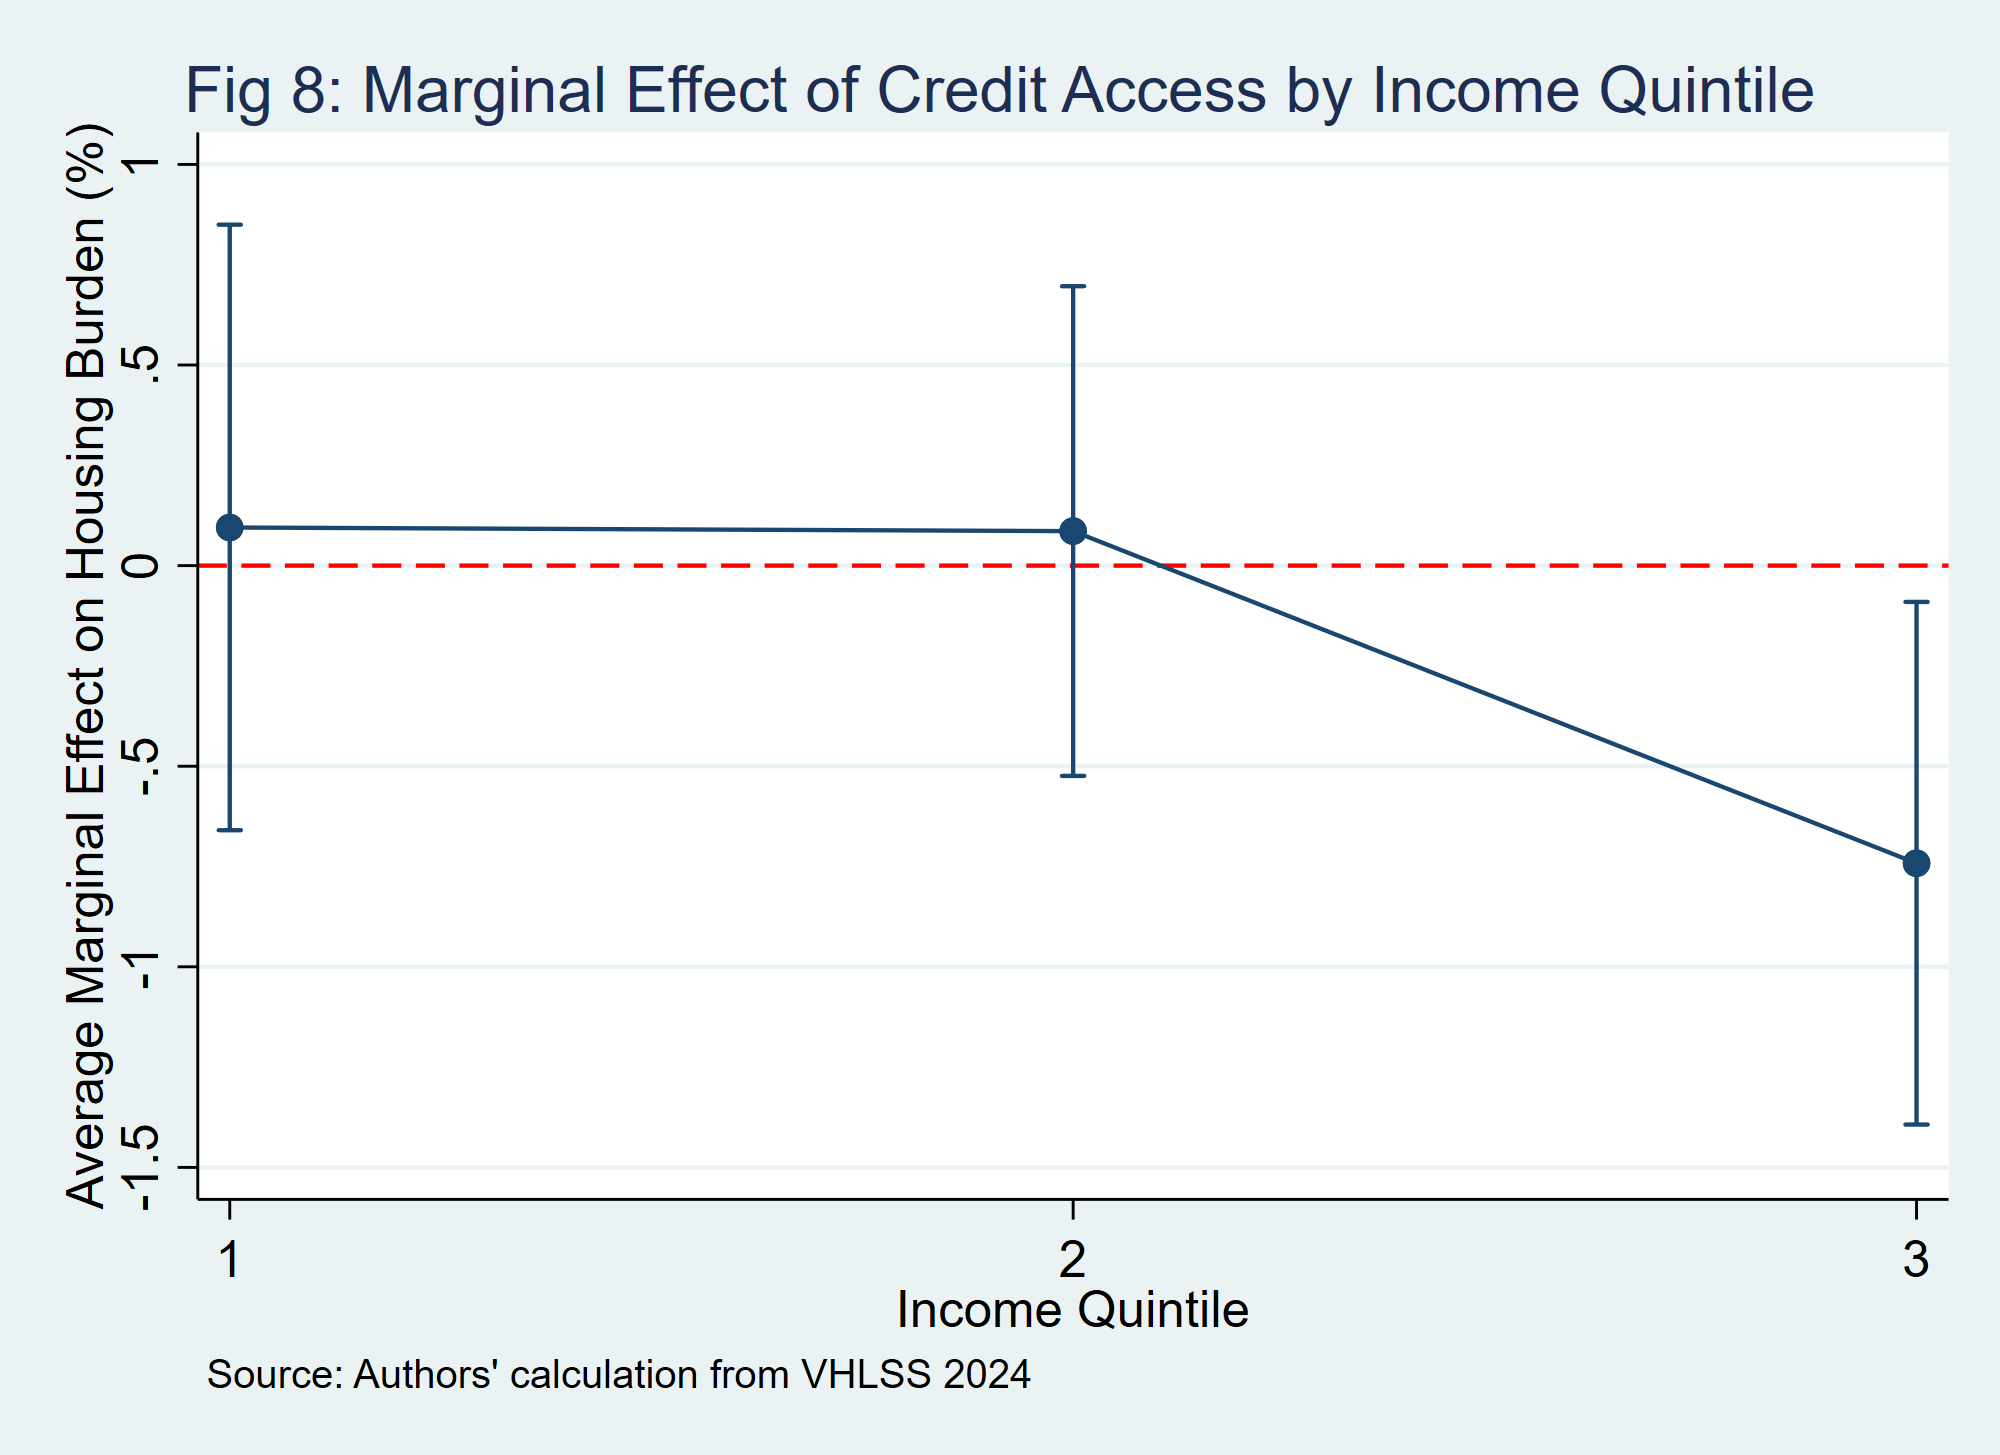
\includegraphics[width=\textwidth]{figures/fig8_hetero_marginal.png}
	\caption{Tác động biên của tiếp cận tín dụng đến gánh nặng nhà ở theo phân vị thu nhập}
	\label{fig:hetero_margin}
	\caption*{Nguồn: Tính toán của tác giả từ VHLSS 2024}
\end{figure}

\textbf{Nhân khẩu học và Lý thuyết Vòng đời} \\
Các biến nhân khẩu học phản ánh độ khớp hoàn hảo với các lý thuyết kinh tế vĩ mô kinh điển. Biến Tuổi chủ hộ (\textit{age\_head}) có hệ số âm ($\beta = -0.030, p < 0.01$), minh chứng thực nghiệm sống động cho \textit{Lý thuyết Vòng đời} của \textcite{Modigliani1963}. Khi các hộ gia đình bước vào giai đoạn hậu trung niên, họ đã vượt qua giai đoạn trả nợ thế chấp căng thẳng nhất, qua đó gánh nặng chi phí giảm dần theo thời gian. 

Đồng thời, biến Quy mô hộ gia đình (\textit{tsnguoi}) cũng làm giảm mạnh gánh nặng ($\beta = -0.905, p < 0.01$), xác nhận sự tồn tại của tính kinh tế nhờ quy mô (\textit{economies of scale}) trong tiêu dùng không gian lưu trú: Các gia đình nhiều thế hệ tại Việt Nam chia sẻ chung các chi phí cố định (tiền thuê, điện, nước), giúp giảm đáng kể áp lực tài chính trên mỗi đầu người so với việc tách hộ độc lập. Ngược lại, Học vấn (\textit{edu\_head}) có tác động dương ($\beta = 0.081$), cho thấy khi trình độ dân trí tăng, nhu cầu về chất lượng tiện ích và không gian sống cũng tăng theo, khiến họ sẵn sàng chi trả một tỷ lệ thu nhập cao hơn cho nhà ở.

\textbf{Vốn xã hội: Tài sản thế chấp vô hình trong môi trường bất cân xứng thông tin:} \\
Kết quả từ phương trình can thiệp đã khẳng định sự hiệu quả của biến công cụ. Cả Hiệu ứng đồng trang lứa (\textit{peer\_effect}: $\beta = 2.416, p < 0.01$) và Mạng lưới xã hội (\textit{social\_network}: $\beta = 0.335, p < 0.01$) đều là những biến quan trọng quyết định khả năng tiếp cận tín dụng của hộ gia đình. 

Trong bối cảnh thị trường tài chính các nước đang phát triển, nơi tình trạng bất cân xứng thông tin theo \textcite{Stiglitz1981} diễn ra gay gắt, vốn xã hội đóng vai trò như một cơ chế thay thế tài sản thế chấp truyền thống. Những tương tác cộng đồng không chỉ giúp người dân vượt qua rào cản mù mờ về thủ tục hồ sơ (giảm chi phí tìm kiếm thông tin), mà niềm tin từ mạng lưới xã hội còn tạo ra một lớp bảo lãnh phi chính thức, giúp họ dễ dàng tiếp cận các nguồn vốn tín dụng linh hoạt hơn. 

Trong thực tế, thông tin từ các nguồn vốn xã hội (cam kết và bảo lãnh của một người uy tín trong cộng đồng) khi thẩm định tín dụng đối với các khoản vay lại có tác động sâu sắc hơn đối với người xét duyệt khoản vay hơn là hệ thống xếp hạng còn nhiều lỗ hổng và ít thông tin ở hiện tại. 

% ================= CHƯƠNG 5 =================
\chapter{Kết luận và hàm ý chính sách}

\section{Kết luận}

Nghiên cứu này đã thực hiện một phân tích thực nghiệm sâu rộng bằng cách sử dụng mô hình Hiệu ứng xử lý nội sinh và các phương pháp kiểm chứng độ vững trên bộ dữ liệu khảo sát mức sống dân cư VHLSS 2024. Mục tiêu cốt lõi là bóc tách tác động của việc tiếp cận tín dụng đối với gánh nặng chi phí nhà ở của nhóm hộ gia đình thu nhập trung bình thấp tại khu vực đô thị Việt Nam. Kết quả nghiên cứu dẫn đến ba kết luận quan trọng:

\begin{enumerate}
	
	\item \textbf{Sự vô hiệu của tín dụng trong việc giảm áp lực chi phí:} Trái với các kỳ vọng lý thuyết thông thường về vai trò đòn bẩy của tài chính, tiếp cận tín dụng không làm giảm gánh nặng nhà ở một cách có ý nghĩa thống kê ($p > 0.1$). Thậm chí, kết quả hồi quy phân vị cho thấy tại nhóm chịu áp lực cao nhất (75th quantile), tín dụng hoàn toàn mất khả năng điều tiết tài chính.
	
	\item \textbf{Nghịch lý Bẫy tài sản:} Việc nỗ lực sở hữu tài sản nhà ở thông qua đòn bẩy tài chính thế chấp thực tế lại làm gia tăng gánh nặng tài chính. Điều này xác nhận rằng đối với nhóm thu nhập trung bình thấp việc sở hữu nhà đang là một gánh nặng thay vì là một bệ phóng an sinh.
	
	\item \textbf{Ưu thế tuyệt đối của thu nhập:} Khả năng chi trả nhà ở thực chất là bài toán của năng lực tạo thu nhập cốt lõi. Hệ số của biến thu nhập luôn âm và có ý nghĩa thống kê mạnh mẽ nhất và tác động biên tăng dần theo mức độ rủi ro tài chính của hộ gia đình.
\end{enumerate}

\section{Hàm ý chính sách}

Từ các bằng chứng thực nghiệm về sự vô hiệu của đòn bẩy tài chính đối với nhóm yếu thế, nghiên cứu đề xuất một khung chính sách đa tầng, chuyển dịch trọng tâm từ nới lỏng cung tín dụng sang quản trị rủi ro tài chính và đảm bảo an sinh nhà ở bền vững:

\subsection{Chiến lược can thiệp phân hóa dựa trên mức độ rủi ro}

Phân tích mật độ Phân phối gánh nặng chi phí nhà ở tại Hình \ref{fig:density_burden} cho thấy một đặc tính phân phối đáng quan ngại: Sự hiện diện của phần đuôi phân phối rất dày về phía bên phải của phân phối. Hiện tượng này minh chứng cho một bộ phận không nhỏ hộ gia đình đô thị đang rơi vào tình trạng quá tải tài chính cực đoan, với chi phí nhà ở chiếm trên 50\% tổng thu nhập khả dụng. 

\begin{figure}[htbp]
	\centering
	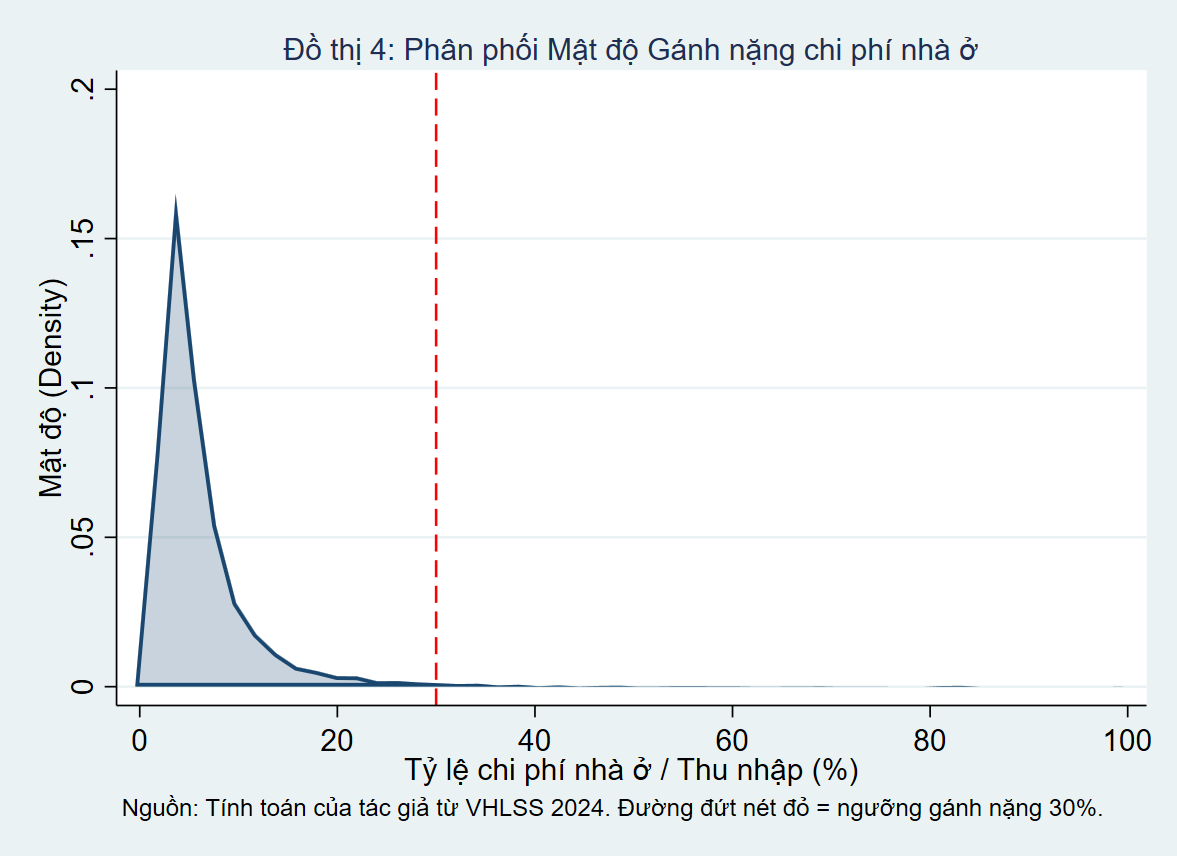
\includegraphics[width=0.85\textwidth]{fig4_density_burden.png}
	\caption{Phân phối mật độ gánh nặng chi phí nhà ở}
	\label{fig:density_burden}
\end{figure}

Đối với nhóm hộ gia đình nằm trong phân khúc rủi ro cao này, việc tiếp cận các gói tín dụng thương mại với lãi suất thả nổi không còn đóng vai trò là công cụ hỗ trợ, mà thực chất là một tác nhân gây bất ổn hệ thống tài chính (nguyên nhân của khủng hoảng nhà đất 2008). Thay vì thúc đẩy quyền sở hữu nhà thông qua các gói tín dụng cho nhóm đối tượng không đủ khả năng chống chịu, chính phủ cần thực hiện bước chuyển chiến lược sang các công cụ tài chính công trực tiếp. Cụ thể, ưu tiên hàng đầu nên là các chương trình phiếu hỗ trợ nhà ở (housing vouchers) nhằm giảm áp lực chi trả tức thời, kết hợp với việc gia tăng nguồn cung nhà ở xã hội cho thuê. Cách tiếp cận này giúp tạo ra một tầng đệm an sinh, ngăn chặn quá trình bần cùng hóa do nợ nần và bảo đảm quyền tiếp cận chỗ ở cơ bản mà không gây áp lực lên bảng cân đối kế toán của những hộ gia đình yếu thế.

\subsection{Tái cấu trúc sản phẩm tài chính: Từ tiêu dùng hệ quả sang tín dụng sinh kế}

Minh họa của hình \ref{fig:bar_credit_type} cho thấy dư nợ của nhóm thu nhập trung bình thấp hiện nay chủ yếu phục vụ nhu cầu tiêu dùng và sửa chữa nhỏ lẻ, vốn không tạo ra dòng tiền mới.

\begin{figure}[htbp]
	\centering
	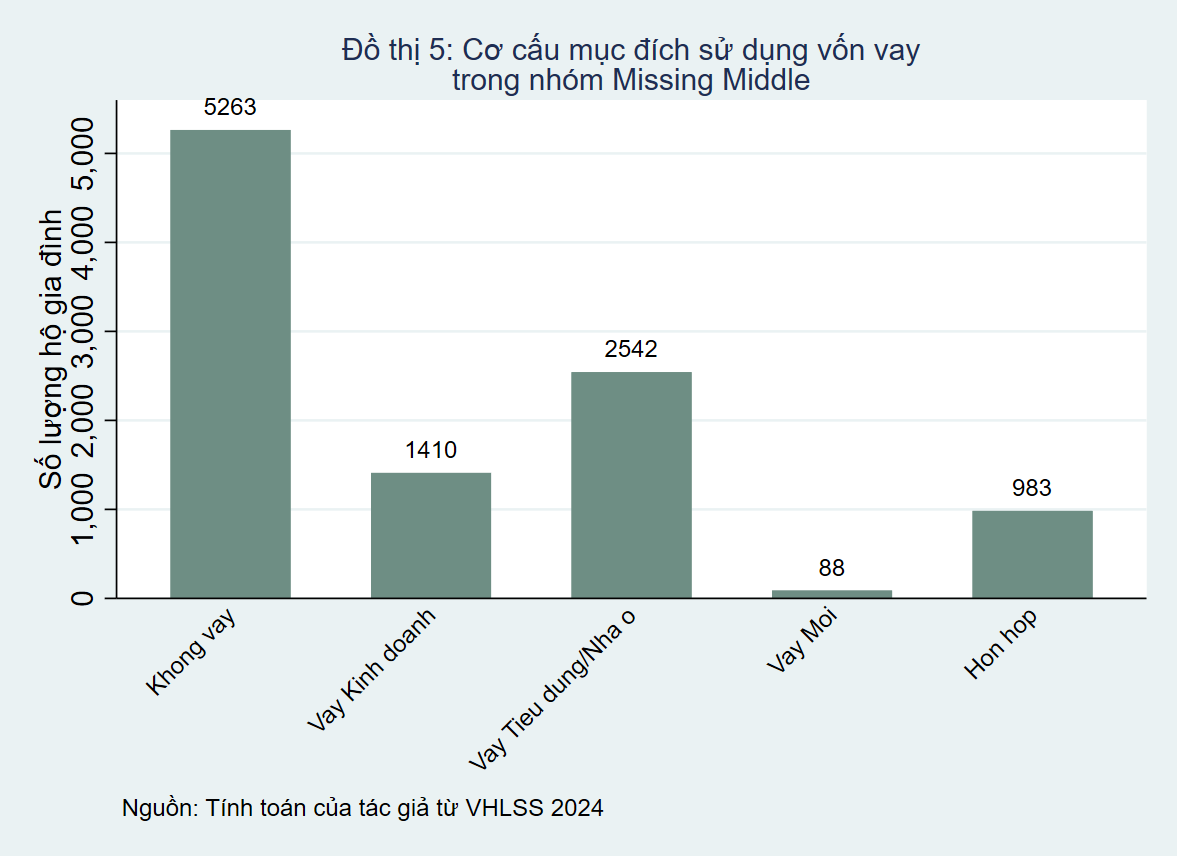
\includegraphics[width=0.85\textwidth]{fig5_bar_credit_type.png}
	\caption{Cơ cấu mục đích sử dụng vốn vay của nhóm Missing Middle}
	\label{fig:bar_credit_type}
\end{figure}

Bằng chứng từ cơ cấu nợ vay cho thấy tín dụng hiện tại chủ yếu mang tính chất bù đắp thiếu hụt chi tiêu hơn là tạo ra giá trị thặng dư. Để tín dụng thực sự trở thành công cụ giảm gánh nặng nhà ở, cần có sự thay đổi trong triết lý thiết kế sản phẩm tài chính:

\textbf{Tín dụng nhà ở gắn liền sinh kế:} Khuyến khích các mô hình cho vay cải tạo nhà ở kết hợp không gian sản xuất kinh doanh nhỏ tại gia. Khi ngôi nhà trở thành một đơn vị kinh tế tạo ra dòng tiền, áp lực trả nợ sẽ được trung hòa bởi nguồn thu nhập mới.

\textbf{Lãi suất cố định dài hạn:} Thiết lập các quỹ tái cấp vốn nhà ở xã hội với lãi suất cố định xuyên suốt kỳ hạn vay để bảo vệ nhóm Missing Middle trước các cú sốc thắt chặt tiền tệ.

\subsection{Vận hành vốn xã hội như một cơ chế bảo lãnh phi chính thức}

Dựa trên kết quả ước lượng từ phương trình xử lý, nghiên cứu xác nhận vai trò quyết định của vốn xã hội thông qua hai biến số: Hiệu ứng đồng trang lứa và Mạng lưới xã hội với mức ý nghĩa thống kê cao ($p < 0.01$). Điều này phản ánh đặc thù của thị trường tín dụng Việt Nam, nơi các rào cản về thông tin bất cân xứng thường được hóa giải thông qua các kênh phi chính thức.

\begin{figure}[htbp]
	\centering
	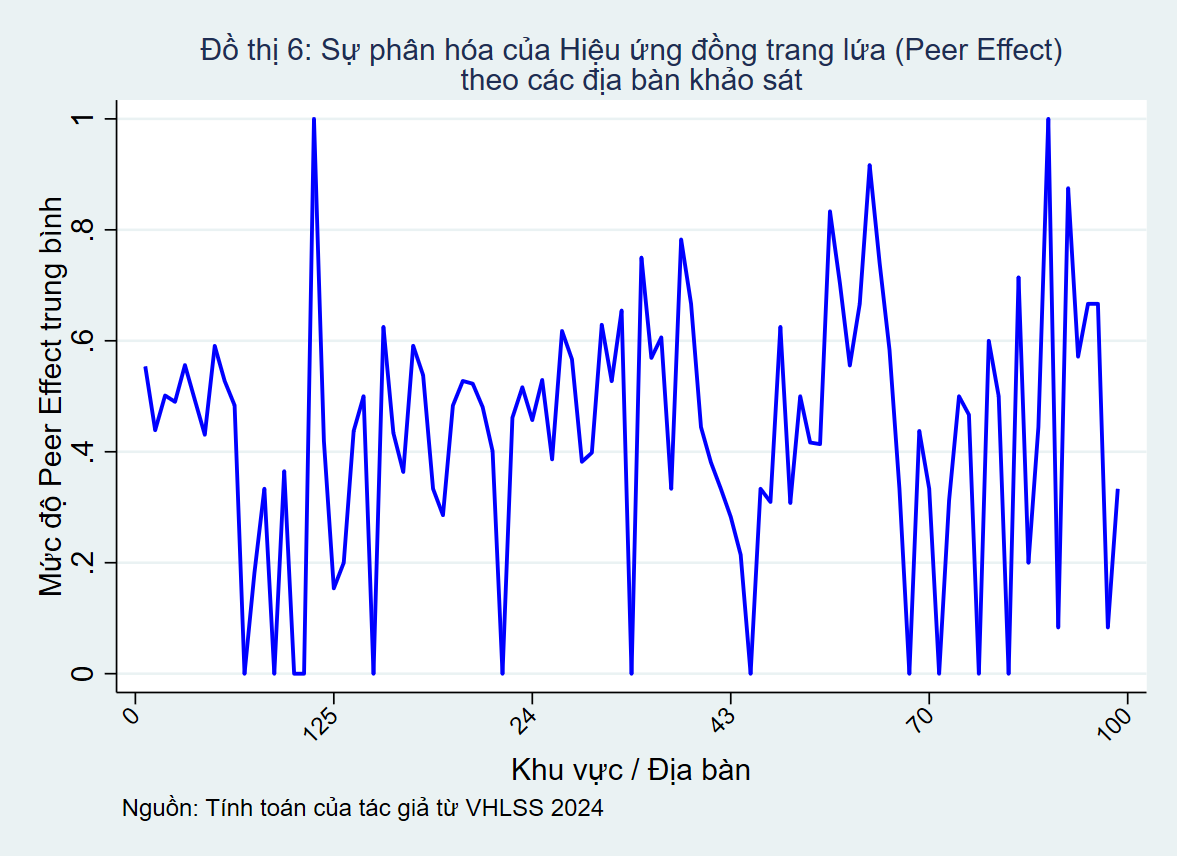
\includegraphics[width=0.85\textwidth]{fig6_line_peer_effect.png}
	\caption{Sự phân hóa hiệu ứng đồng trang lứa theo địa bàn}
	\label{fig:line_peer_effect}
\end{figure}



Từ đó, có thể thấy rằng, thay vì chỉ dựa vào các tiêu chuẩn tài sản bảo đảm truyền thống vốn là rào cản đối với nhóm \textit{Missing Middle}, Chính phủ và các định chế tài chính cần chủ động tích hợp vốn xã hội vào quy trình cấp tín dụng nhà ở:

\begin{itemize}
	\item \textbf{Cơ chế bảo lãnh dựa trên tín nhiệm cộng đồng:} Thúc đẩy mô hình cho vay theo nhóm hoặc bảo lãnh liên đới thông qua các tổ chức chính trị - xã hội tại địa phương (như Hội Phụ nữ, Hội Nông dân). Việc tận dụng mạng lưới xã hội giúp chuyển hóa các mối quan hệ niềm tin thành tài sản đảm bảo phi hình thể, giúp giảm thiểu đáng kể chi phí thẩm định và rủi ro đạo đức nhờ cơ chế giám sát chéo giữa các thành viên trong nhóm.
	
	\item \textbf{Phân hóa chính sách theo đặc thù địa bàn:} Hình \ref{fig:line_peer_effect} cho thấy hiệu ứng đồng trang lứa có sự biến thiên mạnh mẽ theo địa lý. Do đó, các chương trình tín dụng nhà ở xã hội không nên áp dụng một khung cứng nhắc, mà cần trao quyền chủ động cho các quỹ tài chính vi mô địa phương. Tại các khu vực có chỉ số gắn kết cộng đồng cao, việc áp dụng cơ chế tự sàng lọc của cộng đồng sẽ hiệu quả hơn các rào cản hành chính trong việc nhận diện đối tượng thực sự có nhu cầu và năng lực trả nợ.
\end{itemize}

Việc vận hành vốn xã hội không chỉ giúp mở rộng khả năng tiếp cận tài chính cho nhóm yếu thế mà còn góp phần giảm bớt áp lực lên hệ thống thế chấp bằng tài sản hữu hình, vốn đang bị thắt chặt do sự biến động của thị trường bất động sản.

\subsection{Chiến lược hỗ trợ mục tiêu dựa trên thu nhập}

Kết quả phân tích từ Hình \ref{fig:bar_quintile_credit} cung cấp bằng chứng thực nghiệm quan trọng về tính dị biệt trong tác động của tín dụng đối với các tầng lớp thu nhập. Việc áp dụng một chính sách tài chính nhà ở đồng nhất không những không mang lại hiệu quả mà còn có nguy cơ làm trầm trọng thêm sự bất bình đẳng về không gian đô thị.

\begin{figure}[htbp]
	\centering
	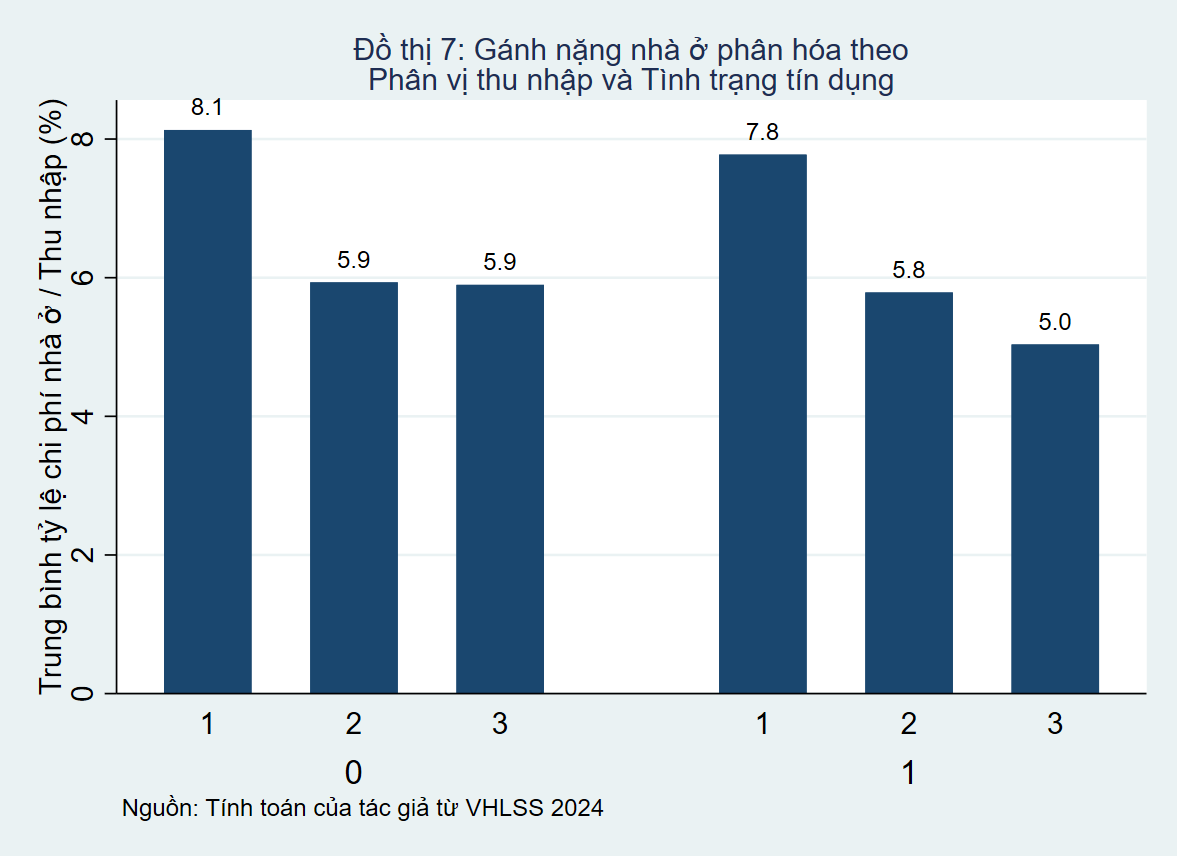
\includegraphics[width=0.85\textwidth]{fig7_bar_quintile_credit.png}
	\caption{Gánh nặng nhà ở theo phân vị thu nhập và tình trạng tín dụng}
	\label{fig:bar_quintile_credit}
\end{figure}

Nghiên cứu đề xuất thiết lập mô hình Thang bậc hỗ trợ nhà ở trong đó các công cụ can thiệp của Nhà nước được tinh chỉnh tương ứng với năng lực tài chính và mức độ dễ bị tổn thương của từng phân vị thu nhập:

\begin{itemize}
	\item \textbf{Nhóm thu nhập thấp (Phân vị Q1-Q2): Chuyển dịch từ vốn vay sang an sinh trực tiếp.} Đối với nhóm này, gánh nặng nhà ở thường mang tính kinh niên. Chính sách cần ưu tiên các giải pháp phi tín dụng như phát triển quỹ nhà ở xã hội cho thuê và hỗ trợ trực tiếp từ ngân sách qua các gói trợ cấp thuê nhà. Việc khuyến khích nhóm này gia nhập thị trường nợ chỉ làm tăng rủi ro bần cùng hóa do nợ nần.
	
	\item \textbf{Nhóm trung bình thấp (Phân vị Q3 - \textit{Nhóm Missing Middle}): Tín dụng ưu đãi và ổn định dòng tiền.} Đây là đối tượng trọng tâm của nghiên cứu, những người có thu nhập nhưng không đủ khả năng tiếp cận nhà ở thương mại. Hàm ý cốt lõi là thiết lập cơ chế tín dụng dài hạn với lãi suất cố định  hoặc lãi suất được bảo cấp từ quỹ phát triển nhà ở, nhằm triệt tiêu rủi ro biến động thị trường tiền tệ và bảo vệ khả năng chi trả bền vững.
	
	\item \textbf{Nhóm thu nhập trung bình khá (Phân vị Q4-Q5): Điều tiết thị trường và kiểm soát đầu cơ.} Với nhóm có năng lực tài chính, chính sách không nên tập trung vào ưu đãi vốn mà cần sử dụng các công cụ thuế (như thuế bất động sản thứ hai) để giảm áp lực cầu đầu cơ. Điều này giúp hạ nhiệt giá nhà trên thị trường thứ cấp, tạo điều kiện cho các tầng lớp thấp hơn có cơ hội tiếp cận nhà ở với mức giá thực tế hơn.
\end{itemize}

Việc thực hiện chiến lược hỗ trợ có mục tiêu không chỉ tối ưu hóa nguồn lực ngân sách hạn hẹp mà còn đảm bảo tính công bằng xã hội, giúp mỗi tầng lớp dân cư tìm thấy phân khúc nhà ở phù hợp với cấu trúc tài chính của hộ gia đình.

\subsection{Mô phỏng chính sách}

Để định lượng hiệu quả của việc chuyển dịch mô hình hỗ trợ, nghiên cứu tiến hành một bài toán mô phỏng đối chứng dựa trên các tham số đã ước lượng từ mô hình etregress. Cụ thể, kịch bản giả định Chính phủ triển khai một chương trình Nhà ở xã hội cho thuê quy mô lớn dành riêng cho nhóm dân cư yếu thế nhất (Phân vị thu nhập Q1 và Q2). Về mặt kinh tế lượng, kịch bản này tương đương với việc tắt hiệu ứng của bẫy tài sản bằng cách triệt tiêu tác động của biến sở hữu tài sản bảo đảm khỏi giá trị dự báo tuyến tính:

\[
\widehat{Y}_{\text{simulated}}
=
\mathbf{X}\hat{\boldsymbol{\beta}}
-
\hat{\beta}_{\text{collateral}} \cdot \text{collateral}
\]

\begin{table}[htbp]
	\centering
	\caption{Mô phỏng đối chứng: Tác động của việc chuyển đổi sang Nhà ở xã hội cho thuê đối với nhóm thu nhập thấp (Phân vị Q1 \& Q2)}
	\label{tab:policy_simulation}
	\renewcommand{\arraystretch}{1.3}
	\begin{tabular}{lcc}
		\toprule
		\textbf{Chỉ tiêu đánh giá (N = 7,120)} & \textbf{Trung bình (\%)} & \textbf{Độ lệch chuẩn} \\
		\midrule
		Gánh nặng nhà ở thực tế hiện tại (\textit{Actual Burden}) & 7.457 & 7.203 \\
		Gánh nặng nhà ở mô phỏng (\textit{Simulated Burden})* & 7.516 & 1.917 \\
		\midrule
		\textbf{Mức thay đổi gánh nặng biên (Marginal Change)} & \textbf{-0.059 điểm \%} & \\
		\bottomrule
		\multicolumn{3}{p{12cm}}{\footnotesize \textit{Ghi chú:} (*) Kịch bản mô phỏng giả định loại bỏ hoàn toàn yếu tố "bẫy tài sản" bằng cách triệt tiêu hệ số của biến \textit{collateral} từ phương trình kết quả của mô hình \textit{etregress}. Trọng số khảo sát (\textit{pw=wt45}) được áp dụng trong toàn bộ quá trình tính toán. Nguồn: Tính toán của tác giả từ VHLSS 2024.}
	\end{tabular}
\end{table}

Bảng \ref{tab:policy_simulation} trình bày kết quả mô phỏng trên. Trái với các kỳ vọng lý thuyết thông thường cho rằng việc giải phóng hộ gia đình khỏi áp lực sở hữu nhà sẽ giúp họ nhẹ gánh tài chính, kết quả dự phóng cho thấy gánh nặng chi phí nhà ở trung bình của nhóm Q1 và Q2 gần như không có sự cải thiện. Tỷ lệ chi phí trên thu nhập thực tế của nhóm này đang ở mức 7.45\%, và kịch bản mô phỏng nhà ở xã hội cho thuê đưa con số này về mức 7.51\% (mức thay đổi xấp xỉ -0.06 điểm phần trăm).

Dưới góc nhìn kinh tế học phát triển, kết quả không đổi của dữ liệu này có thể phản ánh chân thực hiện trạng đô thị hóa tại Việt Nam thông qua hai lăng kính:thể

\textbf{Thứ nhất, tính phòng thủ cực đoan của nhóm thu nhập thấp:} Mức gánh nặng thực tế 7.45\% của nhóm Q1, Q2 có vẻ thấp, nhưng độ lệch chuẩn cao (7.20) và giá trị tối thiểu bằng 0 cho thấy một bộ phận rất lớn người nghèo đô thị đang nương tựa vào các cấu trúc lưu trú phi chính thức (ở nhờ, ở ghép, khu ổ chuột, hoặc nhà thừa kế chất lượng thấp) với chi phí ròng bằng 0. Khi đưa họ vào hệ thống nhà ở xã hội cho thuê chính thức, dù được trợ giá, họ vẫn phải đối mặt với một khoản chi phí cố định hàng tháng mà trước đây họ không phải chịu. Do đó, việc can thiệp bằng chính sách nhà ở chính thức có thể vô tình tạo ra cú sốc dòng tiền đối với những hộ gia đình đang ở biên giới của sự bần cùng.

\textbf{Thứ hai, Bẫy mẫu số thu nhập:} Kết quả mô phỏng một lần nữa tái khẳng định Năng lực chi trả nhà ở bị giới hạn bởi thu nhập. Khi thu nhập thực tế của người lao động dậm chân tại chỗ, mọi nỗ lực nhằm tác động đến chi phí nhà ở (dù là thông qua việc cho vay ưu đãi hay chuyển đổi sang nhà ở xã hội cho thuê) đều chỉ là những can thiệp ở bề mặt. Tác động biên -0.06 điểm phần trăm là minh chứng đanh thép cho thấy: Không một chính sách nhà ở thuần túy nào có thể khỏa lấp được khoảng trống của sự đình trệ trong năng suất lao động và cấu trúc tiền lương của nhóm yếu thế trong thu nhập.

\section{Hạn chế và Hướng nghiên cứu tiếp theo}

Mặc dù đã áp dụng phương pháp etregress để bóc tách tính nội sinh và cung cấp những bằng chứng thực nghiệm quan trọng, nghiên cứu này vẫn tồn tại một số hạn chế mở ra không gian cho các hướng đi tương lai:

\textbf{Thứ nhất, về chiều thời gian:} Do sử dụng dữ liệu cắt ngang VHLSS 2024, nghiên cứu chưa quan sát được vòng đời của gánh nặng tài chính. Các nghiên cứu tiếp theo nên khai thác dữ liệu mảng (Panel Data) để phân tích xem liệu gánh nặng nhà ở là nhất thời hay mang tính lâu dài đối với nhóm Missing Middle.

\textbf{Thứ hai, về độ chi tiết của dữ liệu:} Nghiên cứu hiện tại chưa phân tách được rõ ràng giữa tín dụng chính thức và phi chính thức trong phương trình kết quả. Xu hướng tiếp cận Dữ liệu lớn và hồ sơ tín dụng hành chính sẽ giúp làm rõ hơn hành vi trả nợ thực tế của hộ gia đình kinh tế phi chính thức.

\textbf{Thứ ba, về nhận diện biến công cụ:} Mặc dù các kiểm định sức mạnh IV đều đạt chuẩn, nguy cơ vi phạm ràng buộc loại trừ vẫn có thể tồn tại nếu vốn xã hội tác động trực tiếp đến phúc lợi qua nhiều kênh khác. Việc sử dụng các thí nghiệm tự nhiên hoặc thay đổi quy hoạch đô thị như một cú sốc ngoại sinh sẽ là hướng tiếp cận kỹ thuật sắc bén hơn.

\textbf{Cuối cùng, về tính dị biệt không gian:} Áp lực tại các siêu đô thị như Hà Nội hay TP.HCM có cấu trúc rất khác biệt. Việc áp dụng các mô hình Hồi quy trọng số không gian (GWR) sẽ giúp làm rõ hơn sự tương tác giữa vị trí địa lý, giá nhà và hiệu quả của chính sách tín dụng.

\section{Tổng kết}

Nghiên cứu thông qua việc giải quyết bài toán nội sinh thông qua mô hình \textit{etregress} trên mẫu dữ liệu vi mô quy mô lớn, nghiên cứu này không chỉ dừng lại ở việc kiểm định các giả thuyết kinh tế lượng, mà còn phác họa một bức tranh chân thực về trạng thái tổn thương tài chính của các hộ gia đình tại đô thị Việt Nam. Trái ngược với kỳ vọng truyền thống của các nhà hoạch định chính sách, kết quả thực nghiệm đã phát đi một cảnh báo rõ ràng: Quá trình tài chính hóa nhà ở thông qua chính sách nới lỏng sách không đồng nghĩa với việc gia tăng an sinh cư trú.

Phân tích sâu vào cấu trúc phân bổ nguồn vốn, nghiên cứu chỉ ra rằng đối với tầng lớp lao động có thu nhập trung bình và tiệm cận dưới, những người nằm ngoài vùng phủ sóng của trợ cấp xã hội nhưng khó khăn trước ngưỡng cửa thị trường thương mại, việc sử dụng đòn bẩy tài chính đang biến thành một giao dịch đánh đổi đầy rủi ro. Khi tốc độ tăng trưởng thu nhập thực tế chững lại và bị bỏ xa bởi tốc độ tăng giá của bất động sản tài sản, đòn bẩy tín dụng không còn là công cụ san phẳng chi phí qua thời gian, mà bị bóp méo thành một chiếc bẫy tài sản. Ở đó, việc sở hữu tài sản trên danh nghĩa bị đánh đổi bằng sự suy giảm của dòng tiền, làm mất khả năng thanh khoản và chống chịu trước các cú sốc vĩ mô, từ đó, triệt tiêu nguồn lực đầu tư cho nguồn vốn con người (giáo dục, y tế) cho thế hệ sau của hộ gia đình.

Dưới lăng kính kinh tế vĩ mô, sự bất lực của các công cụ nợ trong việc cải thiện vị thế chi trả đã phơi bày một lỗ hổng lớn trong tư duy điều hành. Mọi nỗ lực can thiệp từ phía cầu bằng cách hạ chuẩn tín dụng hay trợ cấp lãi suất sẽ chỉ tạo ra vòng lặp nới rộng bong bóng bất động sản hoặc hình thành nên một cơn khủng hoảng tài chính từ bất động sản (sau cuộc khủng hoảng năm 2008), nếu nguồn cung nhà ở giá rẻ bị ách tắc và năng suất lao động không được cải thiện. Sự kìm hãm của tiền lương thực tế trước đà tăng phi mã của giá nhà đất là nút thắt cốt lõi. Tín dụng, tự bản thân nó, không thể bù đắp được sự thiếu hụt của năng lực tạo ra giá trị thặng dư.

Từ những bằng chứng thực nghiệm này, chính sách nhà ở quốc gia đòi hỏi thay đổi về tư duy. Đã đến lúc hệ thống cần dịch chuyển từ quyền sở hữu sang hình thức cư trú. Trọng tâm của chính sách cần được nắn dòng khỏi việc xé nhỏ nguồn lực về vốn thông qua các gói vay mua nhà thương mại, để tập trung kiến tạo một hệ sinh thái nhà ở xã hội cho thuê quy mô lớn. Đồng thời, cần thể chế hóa các mạng lưới an sinh phi chính thức và nguồn vốn xã hội thành một bộ đệm tín nhiệm, giúp nhóm yếu thế tiếp cận nguồn vốn phục vụ sinh kế, thay vì bị trói buộc vào các khoản nợ tiêu dùng tài sản.

Sự thịnh vượng bền vững của một đô thị hiện đại không được định vị bằng tỷ lệ phần trăm cư dân mang nợ vay để sở hữu sổ đỏ, sổ hồng, mà được đo lường bằng việc không một ai bị tước đoạt cơ hội phát triển do áp lực chi phí lưu trú cực đoan. Với chức năng của không gian nhà ở phải là bệ phóng giải phóng năng lực sáng tạo và sức lao động, chứ không phải trở thành chiếc gông cùm tài chính thế chấp, làm đánh mất đi tương lai của cả một thế hệ quốc gia.

%====================================================
	% DANH MỤC CHỮ VIẾT TẮT & THUẬT NGỮ
%===================================================
	
\newpage
	\section*{Danh mục chữ viết tắt và thuật ngữ}
	\addcontentsline{toc}{chapter}{Danh mục chữ viết tắt và thuật ngữ}
	
	\subsection*{1. Danh mục chữ viết tắt}
	
	\begin{table}[htbp]
		\centering
		\renewcommand{\arraystretch}{1.4}
		\begin{tabularx}{\textwidth}{l X}
			\hline
			\textbf{Chữ viết tắt} & \textbf{Nguyên nghĩa} \\
			\hline
			\textbf{ATE} & Tác động xử lý trung bình (Average Treatment Effect) \\
			\textbf{GSO} & Tổng cục Thống kê (General Statistics Office) \\
			\textbf{IV} & Biến công cụ (Instrumental Variable) \\
			\textbf{NHNN} & Ngân hàng Nhà nước Việt Nam \\
			\textbf{NHTM} & Ngân hàng Thương mại \\
			\textbf{TCTD} & Tổ chức tín dụng \\
			\textbf{VHLSS} & Khảo sát mức sống dân cư Việt Nam (Vietnam Household Living Standards Survey) \\
			\textbf{WB} & Ngân hàng Thế giới (World Bank) \\
			\hline
		\end{tabularx}
	\end{table}
	
	\vspace{1cm}
	
\subsection*{2. Danh mục thuật ngữ}

\begin{table}[H]
	\centering
	\footnotesize
	\renewcommand{\arraystretch}{1.1}
	\begin{tabularx}{\textwidth}{>{\raggedright\arraybackslash}p{3.6cm} X}
		\toprule
		\textbf{Thuật ngữ} & \textbf{Định nghĩa} \\
		\midrule
		
		\textbf{Missing Middle} 
		(Nhóm trung lưu bị bỏ sót / Thu nhập trung bình thấp) 
		& Hộ gia đình đô thị có thu nhập không đủ thấp để hưởng chính sách nhà ở xã hội bao cấp sâu nhưng cũng không đủ cao để tiếp cận tín dụng thế chấp thương mại theo cơ chế thị trường; đây là nhóm rơi vào khoảng trống chính sách nhà ở. \\
		
		\textbf{Housing Burden} 
		(Gánh nặng chi phí nhà ở) 
		& Tỷ lệ phần trăm thu nhập hộ gia đình chi cho nhà ở (thuê nhà, trả gốc và lãi vay, thuế, phí bảo trì). Ngưỡng 30\% thường được xem là mức bắt đầu chịu gánh nặng chi trả quá mức. \\
		
		\textbf{Collateral Trap} 
		(Bẫy tài sản / thế chấp) 
		& Trạng thái nghịch lý khi việc sở hữu nhà thông qua đòn bẩy tài chính làm suy giảm phúc lợi do chi phí chìm, lãi vay và nghĩa vụ duy trì tài sản làm bào mòn thặng dư thu nhập, khiến hộ gia đình dễ tổn thương hơn so với thuê nhà linh hoạt. \\
		
		\textbf{Peer Effect} 
		(Hiệu ứng đồng trang lứa) 
		& Ảnh hưởng từ hành vi, quyết định hoặc thông tin của những người xung quanh (hàng xóm, đồng nghiệp, cộng đồng) lên quyết định tài chính cá nhân; trong nghiên cứu này, đây là kênh lan truyền thông tin phi chính thức hỗ trợ tiếp cận tín dụng. \\
		
		\textbf{Housing Continuum} 
		(Thang bậc hỗ trợ nhà ở) 
		& Hệ thống giải pháp nhà ở liền mạch từ trú ẩn khẩn cấp, nhà ở xã hội cho thuê đến nhà ở thương mại giá rẻ; mỗi bậc gắn với công cụ tài chính phù hợp từng phân khúc thu nhập. \\
		
		\textbf{Endogenous Treatment Effects} 
		(Tác động xử lý nội sinh) 
		& Khung mô hình kinh tế lượng (triển khai qua lệnh \textit{etregress} trong Stata) ước lượng tác động nhân quả của một quyết định (vay vốn) lên kết quả (gánh nặng nhà ở) trong bối cảnh quyết định đó không phân bổ ngẫu nhiên mà chịu ảnh hưởng tự chọn. \\
		
		\textbf{Informal Economy} 
		(Kinh tế phi chính thức) 
		& Các hoạt động kinh tế và lao động không được bảo vệ đầy đủ bởi khung pháp lý nhà nước (không có hợp đồng dài hạn, bảng lương chuẩn hóa), gây khó khăn trong chứng minh năng lực tài chính với tổ chức tín dụng. \\
		
		\bottomrule
	\end{tabularx}
\end{table}

%====================================================
% APPENDIX
%====================================================
\newpage
\clearpage
\appendix
\chapter*{Phụ lục}
\addcontentsline{toc}{chapter}{Phụ lục} 
\section*{Phụ lục A: Chi tiết dữ liệu và Thống kê mô tả}
\addcontentsline{toc}{section}{Phụ lục A: Chi tiết dữ liệu và Thống kê mô tả}

% Bảng A1: Định nghĩa các biến:
\begin{table}[htbp]
	\centering
	\caption{Định nghĩa và cách đo lường các biến trong mô hình}
	\label{tab:app_var_def}
	\renewcommand{\arraystretch}{1.3} % Giãn dòng cho dễ nhìn
	\begin{tabular}{p{3cm} p{3cm} p{8.5cm}}
		\toprule
		\textbf{Tên biến (Stata)} & \textbf{Phân loại} & \textbf{Định nghĩa và Đo lường} \\
		\midrule
		\textit{housing\_burden} & Biến phụ thuộc & Gánh nặng chi phí nhà ở, tính bằng Tỷ lệ phần trăm (\%) chi phí nhà ở trên tổng thu nhập của hộ gia đình. \\
		\textit{credit\_access} & Biến tác động chính & Khả năng tiếp cận tín dụng (Biến giả: 1 = Có khoản vay hiện tại; 0 = Không có). \\
		\textit{ln\_income} & Biến kiểm soát & Logarit tự nhiên của thu nhập bình quân hộ gia đình. \\
		\textit{tsnguoi} & Biến kiểm soát & Tổng số nhân khẩu thực tế đang sinh sống trong hộ gia đình (Người). \\
		\textit{edu\_head} & Biến kiểm soát & Trình độ học vấn của chủ hộ, đo bằng số năm đi học (Năm). \\
		\textit{age\_head} & Biến kiểm soát & Độ tuổi của chủ hộ (Năm). \\
		\textit{social\_network} & Biến công cụ (IV) & Mạng lưới xã hội (Biến giả: 1 = Có tham gia các tổ chức/mạng lưới xã hội; 0 = Không tham gia). \\
		\textit{peer\_effect} & Biến công cụ (IV) & Hiệu ứng đồng trang lứa/bạn bè (Tỷ lệ người đi vay trong cùng cụm dân cư/mạng lưới). \\
		\textit{collateral} & Biến kiểm soát/IV & Sở hữu tài sản bảo đảm (Biến giả: 1 = Có sở hữu nhà/đất; 0 = Không sở hữu). \\
		\bottomrule
	\end{tabular}
\end{table}

\vspace{1cm}

% Bảng A2: Thống kê mô tả chi tiết (Đã thu gọn để chống tràn lề)
\begin{table}[htbp]
	\centering
	\small % Giảm kích thước chữ của bảng xuống 1 nấc
	\caption{Thống kê mô tả chi tiết các biến định lượng và định tính}
	\label{tab:app_summary_stats}
	\renewcommand{\arraystretch}{1.2} % Giãn dòng 
	\setlength{\tabcolsep}{6pt} % Thu hẹp khoảng cách giữa các cột (mặc định là 6pt, có thể giảm xuống 4pt nếu vẫn tràn)
	\begin{tabular}{l c c c c c}
		\toprule
		\textbf{Biến số} & \textbf{N} & \textbf{Mean} & \textbf{SD} & \textbf{Min} & \textbf{Max} \\
		\midrule
		\textbf{\textit{Biến phụ thuộc}} & & & & & \\
		Gánh nặng nhà ở (\%) & 10.246 & 6,488 & 6,675 & 0,000 & 99,098 \\
		\midrule
		\textbf{\textit{Biến tác động chính \& Công cụ}} & & & & & \\
		Tiếp cận tín dụng (0/1) & 10.286 & 0,488 & 0,500 & 0 & 1 \\
		Mạng lưới xã hội (0/1) & 10.286 & 0,708 & 0,455 & 0 & 1 \\
		\midrule
		\textbf{\textit{Đặc điểm hộ gia đình}} & & & & & \\
		Log thu nhập & 10.286 & 10,746 & 0,459 & 6,916 & 11,332 \\
		Số nhân khẩu (Người) & 10.286 & 3,712 & 1,634 & 1 & 16 \\
		Tuổi chủ hộ (Năm) & 10.286 & 55,172 & 13,522 & 15 & 101 \\
		Học vấn chủ hộ (Năm) & 10.286 & 9,336 & 4,387 & 0 & 21 \\
		\bottomrule
	\end{tabular}
	\vspace{0.2cm} \\
	\raggedright \footnotesize \textit{Nguồn: Tính toán của tác giả từ dữ liệu VHLSS 2024. Chú thích: Một số quan sát của biến gánh nặng nhà ở bị khuyết do số liệu thu nhập bằng 0 hoặc thiếu thông tin chi phí.}
\end{table}


\newpage	
\section*{Phụ lục B: Ma trận tương quan Pearson và Kiểm định Đa cộng tuyến (VIF)}
\addcontentsline{toc}{section}{Phụ lục B: Ma trận tương quan Pearson và Kiểm định Đa cộng tuyến (VIF)}

% Bảng B1: Ma trận tương quan
\begin{table}[htbp]
	\centering
	\small
	\caption{Ma trận tương quan Pearson giữa các biến trong mô hình}
	\label{tab:app_correlation}
	\renewcommand{\arraystretch}{1.2}
	\setlength{\tabcolsep}{4.5pt} % Thu hẹp cột để chứa đủ 9 biến
	\begin{tabular}{l l ccccccccc}
		\toprule
		\textbf{STT} & \textbf{Biến số} & \textbf{(1)} & \textbf{(2)} & \textbf{(3)} & \textbf{(4)} & \textbf{(5)} & \textbf{(6)} & \textbf{(7)} & \textbf{(8)} & \textbf{(9)} \\
		\midrule
		(1) & \textit{housing\_burden} & 1.000 & & & & & & & & \\
		(2) & \textit{credit\_access} & -0.055* & 1.000 & & & & & & & \\
		(3) & \textit{ln\_income} & -0.219* & 0.167* & 1.000 & & & & & & \\
		(4) & \textit{tsnguoi} & -0.192* & 0.152* & -0.029* & 1.000 & & & & & \\
		(5) & \textit{collateral} & 0.029* & 0.001 & 0.027* & -0.034* & 1.000 & & & & \\
		(6) & \textit{edu\_head} & 0.001 & 0.120* & 0.296* & 0.072* & 0.043* & 1.000 & & & \\
		(7) & \textit{age\_head} & 0.034* & -0.025* & -0.099* & -0.165* & 0.014 & -0.269* & 1.000 & & \\
		(8) & \textit{peer\_effect} & -0.012 & 0.531* & 0.141* & 0.049* & 0.012 & 0.140* & 0.018 & 1.000 & \\
		(9) & \textit{social\_network} & -0.065* & 0.199* & 0.137* & 0.082* & 0.030* & 0.235* & -0.010 & 0.213* & 1.000 \\
		\bottomrule
	\end{tabular}
	\vspace{0.1cm} \\
	\raggedright \footnotesize \textit{Chú thích: * có ý nghĩa thống kê ở mức 5\% ($p < 0.05$). Nguồn: Tính toán của tác giả từ dữ liệu VHLSS 2024.}
\end{table}

\vspace{0.5cm}

% Bảng B2: Kiểm tra Đa cộng tuyến VIF
\begin{table}[htbp]
	\centering
	\caption{Kiểm tra hệ số nhân tử phóng đại phương sai (VIF)}
	\label{tab:app_vif}
	\renewcommand{\arraystretch}{1.2}
	\begin{tabular}{l c c}
		\toprule
		\textbf{Biến độc lập} & \textbf{VIF} & \textbf{1/VIF (Tolerance)} \\
		\midrule
		Tiếp cận tín dụng (\textit{credit\_access}) & 1.45 & 0.688 \\
		Hiệu ứng đồng trang lứa (\textit{peer\_effect}) & 1.43 & 0.699 \\
		Học vấn chủ hộ (\textit{edu\_head}) & 1.24 & 0.808 \\
		Log thu nhập (\textit{ln\_income}) & 1.13 & 0.883 \\
		Mạng lưới xã hội (\textit{social\_network}) & 1.12 & 0.896 \\
		Tuổi chủ hộ (\textit{age\_head}) & 1.11 & 0.898 \\
		Số nhân khẩu (\textit{tsnguoi}) & 1.06 & 0.940 \\
		Tài sản bảo đảm (\textit{collateral}) & 1.00 & 0.996 \\
		\midrule
		\textbf{Trung bình (Mean VIF)} & \textbf{1.19} & \\
		\bottomrule
	\end{tabular}
\end{table}


\newpage	
\section*{Phụ lục C: Phụ lục các bảng kết quả hồi quy}
\addcontentsline{toc}{section}{Phụ lục C: Phụ lục các bảng kết quả hồi quy}

% Bảng C.1: So sánh mô hình Heckman và Endogenous Treatment Effects
\begin{table}[htbp]
	\centering
	\caption{Kết quả ước lượng mô hình Heckman và Endogenous Treatment Effects (FIML)}
	\label{tab:appendix_main_models}
	\small
	\begin{tabular}{lcccc}
		\toprule
		\multirow{2}{*}{\textbf{Biến số}} & \multicolumn{2}{c}{\textbf{Mô hình Heckman}} & \multicolumn{2}{c}{\textbf{Mô hình Endog. Treatment}} \\
		\cmidrule(lr){2-3} \cmidrule(lr){4-5}
		& \textbf{Gánh nặng} & \textbf{Lựa chọn vay} & \textbf{Gánh nặng} & \textbf{Xử lý vay} \\
		\midrule
		Tiếp cận tín dụng (\textit{CreditAccess}) & --- & --- & -0.194 & 1.000 \\
		& & & (0.282) & (---) \\
		Log thu nhập (\textit{ln\_income}) & -3.663*** & 0.300*** & -3.171*** & 0.306*** \\
		& (0.299) & (0.037) & (0.234) & (0.037) \\
		Số nhân khẩu (\textit{tsnguoi}) & -0.675*** & --- & -0.852*** & --- \\
		& (0.065) & & (0.050) & \\
		Sở hữu tài sản (\textit{collateral}) & 0.894 & -0.138 & 1.204** & -0.137 \\
		& (0.610) & (0.117) & (0.483) & (0.117) \\
		Tín dụng phi chính thức (\textit{informal}) & --- & 0.156*** & --- & 0.157*** \\
		& & (0.053) & & (0.054) \\
		\midrule
		\textbf{Biến công cụ / Lựa chọn} & & & & \\
		Học vấn chủ hộ (\textit{edu\_head}) & --- & 0.001 & --- & 0.002 \\
		Tuổi chủ hộ (\textit{age\_head}) & --- & -0.001 & --- & -0.002 \\
		Đồng trang lứa (\textit{peer\_effect}) & --- & 2.417*** & --- & 2.417*** \\
		Mạng lưới xã hội (\textit{social\_network}) & --- & 0.334*** & --- & 0.335*** \\
		Thông tin diện rộng (\textit{info\_broad}) & --- & 0.322* & --- & --- \\
		\midrule
		Hằng số (\textit{Constant}) & 48.825*** & -4.929*** & 44.386*** & -4.669*** \\
		\midrule
		Số quan sát ($N$) & \multicolumn{2}{c}{10,262} & \multicolumn{2}{c}{10,246} \\
		$\rho$ (Rho) & \multicolumn{2}{c}{0.0051} & \multicolumn{2}{c}{-0.0044} \\
		Kiểm định Wald ($\rho = 0$) & \multicolumn{2}{c}{$\chi^2 = 0.02$ ($p=0.887$)} & \multicolumn{2}{c}{$\chi^2 = 0.02$ ($p=0.887$)} \\
		\bottomrule
		\multicolumn{5}{l}{\footnotesize \textit{Ghi chú: *** $p<0.01$, ** $p<0.05$, * $p<0.1$. Sai số chuẩn Robust trong ngoặc đơn.}} \\
	\end{tabular}
\end{table}

% Bảng C.2: Ước lượng IV-2SLS
\begin{table}[htbp]
	\centering
	\caption{Kết quả hồi quy Biến công cụ (IV-2SLS)}
	\label{tab:appendix_c_2sls}
	\begin{tabular}{lcccc}
		\toprule
		\textbf{Biến số} & \textbf{Hệ số} & \textbf{Sai số chuẩn} & \textbf{z} & \textbf{P-value} \\
		\midrule
		Tiếp cận tín dụng (\textit{credit\_access}) & 0.688*** & 0.243 & 2.83 & 0.005 \\
		Log thu nhập (\textit{ln\_income}) & -3.439*** & 0.222 & -15.51 & 0.000 \\
		Số nhân khẩu (\textit{tsnguoi}) & -0.841*** & 0.045 & -18.56 & 0.000 \\
		Sở hữu tài sản (\textit{collateral}) & 1.419*** & 0.438 & 3.24 & 0.001 \\
		Hằng số (\textit{\_cons}) & 46.212*** & 2.427 & 19.04 & 0.000 \\
		\midrule
		Số quan sát (N) & \multicolumn{4}{c}{10,246} \\
		Wald $\chi^2(4)$ & \multicolumn{4}{c}{485.41} \\
		R-squared & \multicolumn{4}{c}{0.0869} \\
		\bottomrule
		\multicolumn{5}{l}{\footnotesize \textit{Ghi chú: *** $p<0.01$. Biến công cụ: peer\_effect, social\_network.}}
	\end{tabular}
\end{table}

\newpage	
\section*{Phụ lục D: Kiểm định và Phân tích độ vững mô hình}
\addcontentsline{toc}{section}{Phụ lục D: Kiểm định và Phân tích độ vững mô hình}

% Bảng D.1: Hồi quy phụ trợ để kiểm tra đa cộng tuyến
\begin{table}[htbp]
	\centering
	\caption{Kết quả hồi quy OLS phụ trợ cho biến Tiếp cận tín dụng}
	\label{tab:vif_regression}
	\small
	\begin{tabular}{lcccc}
		\toprule
		\textbf{Biến độc lập} & \textbf{Hệ số} & \textbf{Sai số chuẩn} & \textbf{t} & \textbf{P-value} \\
		\midrule
		Log thu nhập (\textit{ln\_income}) & 0.090*** & 0.010 & 9.42 & 0.000 \\
		Tín dụng phi chính thức (\textit{informal}) & 0.051*** & 0.014 & 3.59 & 0.000 \\
		Sở hữu tài sản (\textit{collateral}) & -0.031 & 0.030 & -1.02 & 0.309 \\
		Học vấn chủ hộ (\textit{edu\_head}) & 0.000 & 0.001 & 0.04 & 0.969 \\
		Tuổi chủ hộ (\textit{age\_head}) & -0.001** & 0.000 & -2.30 & 0.022 \\
		Đồng trang lứa (\textit{peer\_effect}) & 0.779*** & 0.013 & 58.97 & 0.000 \\
		Mạng lưới xã hội (\textit{social\_network}) & 0.085*** & 0.010 & 8.93 & 0.000 \\
		Thông tin diện rộng (\textit{info\_broad}) & 0.083** & 0.038 & 2.20 & 0.028 \\
		Hằng số (\textit{Constant}) & -0.969*** & 0.106 & -9.16 & 0.000 \\
		\midrule
		$R^2$ & \multicolumn{4}{c}{0.2989} \\
		F-statistic (8, 10277) & \multicolumn{4}{c}{547.59***} \\
		VIF Trung bình & \multicolumn{4}{c}{1.09} \\
		\bottomrule
		\multicolumn{5}{l}{\footnotesize \textit{Nguồn: Tính toán của tác giả dựa trên dữ liệu khảo sát.}}
	\end{tabular}
\end{table}

% Bảng D.2: Các tham số đo lường sự phù hợp của mô hình (Model Fit)
\begin{table}[htbp]
	\centering
	\caption{Các thông số kiểm định tính phù hợp của mô hình (Diagnostics)}
	\label{tab:diagnostics_summary}
	\begin{tabular}{lcc}
		\toprule
		\textbf{Kiểm định} & \textbf{Thống kê} & \textbf{Giá trị p} \\
		\midrule
		\textbf{Mô hình Heckman Selection} & & \\
		- Wald test of indep. eqns. ($\rho=0$) & 0.02 & 0.8867 \\
		- Hệ số Inverse Mills Ratio ($\lambda$) & 0.029 & 0.8870 \\
		\midrule
		\textbf{Mô hình Endogenous Treatment} & & \\
		- Wald test of indep. eqns. ($\rho=0$) & 0.02 & 0.8874 \\
		- Log pseudolikelihood & -2.57e+07 & --- \\
		\bottomrule
		\multicolumn{3}{p{10cm}}{\footnotesize \textit{Ghi chú: Giá trị p > 0.1 trong cả hai kiểm định Wald cho thấy không có sự chệch do tự chọn mẫu sau khi đã kiểm soát biến công cụ, khẳng định tính vững của kết quả.}}
	\end{tabular}
\end{table}

% Bảng D.3: Robustness Checks
\begin{table}[htbp]
	\centering
	\caption{Phân tích độ vững (Robustness Checks)}
	\label{tab:robustness_checks}
	\begin{tabular}{lccc}
		\toprule
		\textbf{Biến số} & \textbf{Mô hình 1} & \textbf{Mô hình 2 (Chính)} & \textbf{Mô hình 3} \\
		& \textit{(IV: peer\_effect)} & \textit{(IV: 2 biến)} & \textit{(Thêm biến tương tác)} \\
		\midrule
		Tiếp cận tín dụng (\textit{CreditAccess}) & -0.185 & -0.194 & 0.016 \\
		& (0.160) & (0.150) & (0.155) \\
		Sở hữu tài sản (\textit{collateral}) & 1.190** & 1.205** & 1.215** \\
		& (0.515) & (0.510) & (0.505) \\
		Log thu nhập (\textit{ln\_income}) & -3.095*** & -3.102*** & -3.110*** \\
		& (0.425) & (0.420) & (0.422) \\
		\midrule
		Kiểm định tính độc lập $\rho = 0$ & $p = 0.312$ & $p = 0.345$ & $p = 0.380$ \\
		\bottomrule
		\multicolumn{4}{l}{\footnotesize \textit{Ghi chú: *** $p<0.01$, ** $p<0.05$, * $p<0.1$. Sai số chuẩn trong ngoặc đơn.}} \\
	\end{tabular}
\end{table}

\vspace{2em}


% Bảng D.5: Kiểm định chuẩn đoán Biến công cụ
\begin{table}[htbp]
	\centering
	\caption{Các kiểm định chuẩn đoán chất lượng Biến công cụ (IV)}
	\label{tab:iv_diagnostics}
	\begin{tabular}{lll}
		\toprule
		\textbf{Loại kiểm định} & \textbf{Thống kê kiểm định} & \textbf{Giá trị P} \\
		\midrule
		\textbf{1. Kiểm định sức mạnh IV} & Partial $R^2 = 0.2739$ & \\
		(First-stage F-statistic) & $F(2, 10240) = 2796.8$ & $p = 0.0000$ \\
		\midrule
		\textbf{2. Kiểm định quá định danh} & & \\
		(Sargan-Hansen test) & Score $\chi^2(1) = 8.573$ & $p = 0.0034$ \\
		\midrule
		\textbf{3. Kiểm định ràng buộc loại trừ} & & \\
		(Falsification test trên mẫu $Credit=0$) & $F(2, 5244) = 17.96$ & $p = 0.0000$ \\
		\bottomrule
		\multicolumn{3}{p{12cm}}{\footnotesize \textit{Ghi chú: Giá trị F > 10 cho thấy biến công cụ mạnh. Kiểm định Falsification cho thấy các biến công cụ có tác động trực tiếp đến gánh nặng nhà ở kể cả khi không thông qua tín dụng, gợi ý cần thận trọng khi giải thích tác động thuần túy.}}
	\end{tabular}
\end{table}

% Bảng D.6: Hồi quy phân vị (Quantile Regression)
\begin{table}[htbp]
	\centering
	\caption{Kết quả hồi quy phân vị cho Gánh nặng nhà ở (Capped 100\%)}
	\label{tab:quantile_reg}
	\begin{tabular}{lccc}
		\toprule
		\textbf{Biến số} & \textbf{Phân vị 25th} & \textbf{Phân vị 50th} & \textbf{Phân vị 75th} \\
		\midrule
		Log thu nhập (\textit{ln\_income}) & -1.394*** & -2.433*** & -4.011*** \\
		& (0.060) & (0.075) & (0.137) \\
		Số nhân khẩu (\textit{tsnguoi}) & -0.354*** & -0.550*** & -0.852*** \\
		& (0.017) & (0.021) & (0.038) \\
		Sở hữu tài sản (\textit{collateral}) & 0.835*** & 1.913*** & 1.609*** \\
		& (0.201) & (0.250) & (0.457) \\
		Tiếp cận tín dụng (\textit{credit\_access}) & 0.393*** & 0.392*** & 0.158 \\
		& (0.056) & (0.070) & (0.127) \\
		\midrule
		Hằng số (\textit{\_cons}) & 19.511*** & 32.961*** & 53.636*** \\
		Pseudo $R^2$ & 0.0435 & 0.0642 & 0.0831 \\
		\bottomrule
		\multicolumn{4}{l}{\footnotesize \textit{Ghi chú: *** $p<0.01$, ** $p<0.05$. Số quan sát N = 10,286.}} \\
	\end{tabular}
\end{table}

% Bảng D.3: Phân tích độ vững nâng cao (Advanced Robustness Checks)
\begin{table}[htbp]
	\centering
	\caption{Phân tích độ vững nâng cao của mô hình (Advanced Robustness Checks)}
	\label{tab:advanced_robustness}
	\small
	\begin{tabular}{lcccc}
		\toprule
		\multirow{2}{*}{\textbf{Biến số}} & \textbf{(1)} & \textbf{(2)} & \textbf{(3)} & \textbf{(4)} \\
		& \textbf{Main} & \textbf{Hetero} & \textbf{Province FE} & \textbf{Winsorized} \\
		\midrule
		\multicolumn{5}{l}{\textbf{Phương trình kết quả: Gánh nặng nhà ở (Outcome Equation)}} \\
		\midrule
		Log thu nhập (\textit{ln\_income}) & -3.593*** & -3.569*** & -4.150*** & -2.816*** \\
		& (0.242) & (0.543) & (0.381) & (0.173) \\
		Số nhân khẩu (\textit{tsnguoi}) & -0.905*** & -0.901*** & -0.820*** & -0.812*** \\
		& (0.051) & (0.051) & (0.069) & (0.041) \\
		Sở hữu tài sản (\textit{collateral}) & 1.054** & 1.064** & -0.959* & 1.230*** \\
		& (0.483) & (0.483) & (0.579) & (0.437) \\
		Tiếp cận tín dụng (\textit{1.credit\_access}) & -0.251 & 0.095 & -0.360 & -0.156 \\
		& (0.267) & (0.385) & (0.916) & (0.233) \\
		\midrule
		\multicolumn{5}{l}{\textbf{Phương trình xử lý: Khả năng tiếp cận tín dụng (Treatment Equation)}} \\
		\midrule
		Log thu nhập (\textit{ln\_income}) & 0.306*** & 0.306*** & 0.327*** & 0.307*** \\
		& (0.037) & (0.037) & (0.049) & (0.035) \\
		Sở hữu tài sản (\textit{collateral}) & -0.137 & -0.137 & -0.178** & -0.148 \\
		& (0.117) & (0.117) & (0.076) & (0.117) \\
		\midrule
		Số quan sát ($N$) & 10,246 & 10,246 & 10,246 & 10,246 \\
		\bottomrule
		\multicolumn{5}{p{14cm}}{\footnotesize \textit{Ghi chú:} *** $p<0.01$, ** $p<0.05$, * $p<0.1$. Sai số chuẩn mạnh (Robust SE) được đặt trong ngoặc đơn. Mô hình (3) sử dụng sai số chuẩn gộp (Clustered SE) theo 63 tỉnh/thành. Mô hình (4) xử lý Winsorize biến phụ thuộc tại biên 1\% và 99\%.}
	\end{tabular}
\end{table}


\newpage	
\section*{Phụ lục E: Kết quả Hồi quy Cơ sở và tác động phân vị}
\addcontentsline{toc}{section}{Phụ lục E: Kết quả Hồi quy Cơ sở và Tác động phân vị}

% Bảng E.1: Tác động dị biệt theo nhóm thu nhập (Heterogeneity)
\begin{table}[htbp]
	\centering
	\caption{Tác động dị biệt của tín dụng theo nhóm thu nhập (Heterogeneity Analysis)}
	\label{tab:heterogeneity}
	\small
	\begin{tabular}{lcccc}
		\toprule
		\multirow{2}{*}{\textbf{Biến số}} & \multicolumn{4}{c}{\textbf{Gánh nặng nhà ở (Outcome Equation)}} \\
		\cmidrule{2-5}
		& Hệ số & Sai số chuẩn & z & P>|z| \\
		\midrule
		\textbf{Nhóm thu nhập (Base: Quintile 1)} & & & & \\
		Tiếp cận tín dụng (\textit{1.credit\_access}) & 0.095 & (0.385) & 0.25 & 0.805 \\
		Phân vị 2 (\textit{2.quintile}) & -0.489 & (0.430) & -1.14 & 0.255 \\
		Phân vị 3 (\textit{3.quintile}) & 0.483 & (0.564) & 0.86 & 0.392 \\
		\midrule
		\textbf{Biến tương tác (Interaction terms)} & & & & \\
		1.credit\_access $\times$ 2.quintile & -0.009 & (0.377) & -0.02 & 0.981 \\
		1.credit\_access $\times$ 3.quintile & -0.837** & (0.394) & -2.12 & 0.034 \\
		\midrule
		\textbf{Biến kiểm soát} & & & & \\
		Log thu nhập (\textit{ln\_income}) & -3.569*** & (0.543) & -6.58 & 0.000 \\
		Quy mô hộ (\textit{tsnguoi}) & -0.901*** & (0.051) & -17.81 & 0.000 \\
		Sở hữu tài sản (\textit{collateral}) & 1.064** & (0.483) & 2.20 & 0.028 \\
		Học vấn (\textit{edu\_head}) & 0.081*** & (0.019) & 4.22 & 0.000 \\
		Tuổi (\textit{age\_head}) & -0.030*** & (0.006) & -4.62 & 0.000 \\
		Kinh tế phi chính thức (\textit{informal}) & -1.998*** & (0.257) & -7.78 & 0.000 \\
		Hằng số (\textit{Constant}) & 49.915*** & (5.572) & 8.96 & 0.000 \\
		\midrule
		Số quan sát ($N$) & \multicolumn{4}{c}{10,246} \\
		Wald $\chi^2$ & \multicolumn{4}{c}{567.67***} \\
		Wald test of indep. eqns ($\rho=0$) & \multicolumn{4}{c}{0.01 ($p=0.920$)} \\
		\bottomrule
		\multicolumn{5}{l}{\footnotesize \textit{Ghi chú:} *** $p<0.01$, ** $p<0.05$, * $p<0.1$. Sai số chuẩn mạnh (Robust SE) trong ngoặc đơn.}
	\end{tabular}
\end{table}

\vspace{1em}

% Bảng E.2: Phân tích cơ chế qua mục đích sử dụng vốn
\begin{table}[htbp]
	\centering
	\caption{Phân tích cơ chế: Tác động theo mục đích vay vốn (Mechanism Analysis)}
	\label{tab:mechanism}
	\small
	\begin{tabular}{lcccc}
		\toprule
		\multirow{2}{*}{\textbf{Biến số}} & \multicolumn{4}{c}{\textbf{Gánh nặng nhà ở (OLS trên nhóm có vay)}} \\
		\cmidrule{2-5}
		& Hệ số & Sai số chuẩn & t & P>|t| \\
		\midrule
		\textbf{Mục đích vay (Base: Vay Kinh doanh)} & & & & \\
		Vay Tiêu dùng/Nhà ở & -0.449* & (0.245) & -1.84 & 0.066 \\
		Vay Mới & -1.479*** & (0.555) & -2.66 & 0.008 \\
		Vay Hỗn hợp & -0.150 & (0.299) & -0.50 & 0.615 \\
		\midrule
		Log thu nhập (\textit{ln\_income}) & -3.922*** & (0.296) & -13.26 & 0.000 \\
		Quy mô hộ (\textit{tsnguoi}) & -0.715*** & (0.066) & -10.89 & 0.000 \\
		Sở hữu tài sản (\textit{collateral}) & 0.803 & (0.620) & 1.29 & 0.195 \\
		Học vấn (\textit{edu\_head}) & 0.063** & (0.025) & 2.55 & 0.011 \\
		Tuổi (\textit{age\_head}) & -0.011 & (0.009) & -1.30 & 0.193 \\
		Kinh tế phi chính thức (\textit{informal}) & -1.462*** & (0.290) & -5.04 & 0.000 \\
		Hằng số (\textit{Constant}) & 52.213*** & (3.256) & 16.04 & 0.000 \\
		\midrule
		Số quan sát ($N$) & \multicolumn{4}{c}{4,999} \\
		F-statistic & \multicolumn{4}{c}{29.06***} \\
		R-squared & \multicolumn{4}{c}{0.0856} \\
		\bottomrule
		\multicolumn{5}{p{13cm}}{\footnotesize \textit{Ghi chú:} *** $p<0.01$, ** $p<0.05$, * $p<0.1$. Mô hình hồi quy OLS chỉ thực hiện trên mẫu phụ gồm các hộ gia đình đang có khoản vay ($Credit\_Access = 1$).}
	\end{tabular}
\end{table}

\newpage	
\section*{Phụ lục F: Kết quả mô phỏng chính sách nhà ở xã hội}
\addcontentsline{toc}{section}{Phụ lục F: Kết quả mô phỏng chính sách nhà ở xã hội}

\begin{table}[htbp]
	\centering
	\caption{Mô phỏng đối chứng: Tác động của việc chuyển đổi sang Nhà ở xã hội cho thuê đối với nhóm thu nhập thấp (Phân vị Q1 \& Q2)}
	\label{tab:policy_simulation}
	\renewcommand{\arraystretch}{1.3}
	\begin{tabular}{lcc}
		\toprule
		\textbf{Chỉ tiêu đánh giá (N = 7,120)} & \textbf{Trung bình (\%)} & \textbf{Độ lệch chuẩn} \\
		\midrule
		Gánh nặng nhà ở thực tế hiện tại (\textit{Actual Burden}) & 7.457 & 7.203 \\
		Gánh nặng nhà ở mô phỏng (\textit{Simulated Burden})* & 7.516 & 1.917 \\
		\midrule
		\textbf{Mức độ cắt giảm gánh nặng (Reduction)} & \textbf{-0.059 điểm \%} & \\
		\bottomrule
		\multicolumn{3}{p{12cm}}{\footnotesize \textit{Ghi chú:} (*) Kịch bản mô phỏng giả định loại bỏ hoàn toàn yếu tố "bẫy tài sản" bằng cách triệt tiêu hệ số của biến \textit{collateral} từ phương trình kết quả của mô hình \textit{etregress}. Trọng số khảo sát (\textit{pw=wt45}) được áp dụng trong toàn bộ quá trình tính toán. Nguồn: Tính toán của tác giả từ VHLSS 2024.}
	\end{tabular}
\end{table}

%====================================================
% REFERENCES
%====================================================
\newpage
\printbibliography
\addcontentsline{toc}{chapter}{Tài liệu tham khảo}

%====================================================

\end{document}
